% Options for packages loaded elsewhere
\PassOptionsToPackage{unicode}{hyperref}
\PassOptionsToPackage{hyphens}{url}
%
\documentclass[
  a4paper,
]{scrbook}

\usepackage{amsmath,amssymb}
\usepackage{iftex}
\ifPDFTeX
  \usepackage[T1]{fontenc}
  \usepackage[utf8]{inputenc}
  \usepackage{textcomp} % provide euro and other symbols
\else % if luatex or xetex
  \usepackage{unicode-math}
  \defaultfontfeatures{Scale=MatchLowercase}
  \defaultfontfeatures[\rmfamily]{Ligatures=TeX,Scale=1}
\fi
\usepackage{lmodern}
\ifPDFTeX\else  
    % xetex/luatex font selection
  \setmainfont[]{Latin Modern Roman}
  \setsansfont[]{Latin Modern Roman}
\fi
% Use upquote if available, for straight quotes in verbatim environments
\IfFileExists{upquote.sty}{\usepackage{upquote}}{}
\IfFileExists{microtype.sty}{% use microtype if available
  \usepackage[]{microtype}
  \UseMicrotypeSet[protrusion]{basicmath} % disable protrusion for tt fonts
}{}
\makeatletter
\@ifundefined{KOMAClassName}{% if non-KOMA class
  \IfFileExists{parskip.sty}{%
    \usepackage{parskip}
  }{% else
    \setlength{\parindent}{0pt}
    \setlength{\parskip}{6pt plus 2pt minus 1pt}}
}{% if KOMA class
  \KOMAoptions{parskip=half}}
\makeatother
\usepackage{xcolor}
\setlength{\emergencystretch}{3em} % prevent overfull lines
\setcounter{secnumdepth}{5}
% Make \paragraph and \subparagraph free-standing
\ifx\paragraph\undefined\else
  \let\oldparagraph\paragraph
  \renewcommand{\paragraph}[1]{\oldparagraph{#1}\mbox{}}
\fi
\ifx\subparagraph\undefined\else
  \let\oldsubparagraph\subparagraph
  \renewcommand{\subparagraph}[1]{\oldsubparagraph{#1}\mbox{}}
\fi


\providecommand{\tightlist}{%
  \setlength{\itemsep}{0pt}\setlength{\parskip}{0pt}}\usepackage{longtable,booktabs,array}
\usepackage{calc} % for calculating minipage widths
% Correct order of tables after \paragraph or \subparagraph
\usepackage{etoolbox}
\makeatletter
\patchcmd\longtable{\par}{\if@noskipsec\mbox{}\fi\par}{}{}
\makeatother
% Allow footnotes in longtable head/foot
\IfFileExists{footnotehyper.sty}{\usepackage{footnotehyper}}{\usepackage{footnote}}
\makesavenoteenv{longtable}
\usepackage{graphicx}
\makeatletter
\def\maxwidth{\ifdim\Gin@nat@width>\linewidth\linewidth\else\Gin@nat@width\fi}
\def\maxheight{\ifdim\Gin@nat@height>\textheight\textheight\else\Gin@nat@height\fi}
\makeatother
% Scale images if necessary, so that they will not overflow the page
% margins by default, and it is still possible to overwrite the defaults
% using explicit options in \includegraphics[width, height, ...]{}
\setkeys{Gin}{width=\maxwidth,height=\maxheight,keepaspectratio}
% Set default figure placement to htbp
\makeatletter
\def\fps@figure{htbp}
\makeatother

\usepackage{booktabs}
\usepackage{longtable}
\usepackage{array}
\usepackage{multirow}
\usepackage{wrapfig}
\usepackage{float}
\usepackage{colortbl}
\usepackage{pdflscape}
\usepackage{tabu}
\usepackage{threeparttable}
\usepackage{threeparttablex}
\usepackage[normalem]{ulem}
\usepackage{makecell}
\usepackage{xcolor}
\usepackage{titling}
\setlength{\droptitle}{-2cm}
\preauthor{
  \begin{center}
  \Large
  \vspace{10mm}
  by

  \vspace{20mm}
}
\postauthor{
  \end{center}
  \vfill
}

\predate{
  \begin{center}
  A thesis 
  submitted in fulfilment of the \\
  requirements of the degree of \\
  Doctor of Philosophy in Physics\\               % Degree
  School of Physical and Chemical Sciences\\          % Department
  Te Herenga Waka - Victoria University of Wellington\\                       % University 
  \vspace{5mm}
}
\postdate{
  \\
  
\includegraphics[width=3in,height=1.5in]{figures/VUW-logo.png}\\
  \end{center}
  }
\makeatletter
\makeatother
\makeatletter
\@ifpackageloaded{bookmark}{}{\usepackage{bookmark}}
\makeatother
\makeatletter
\@ifpackageloaded{caption}{}{\usepackage{caption}}
\AtBeginDocument{%
\ifdefined\contentsname
  \renewcommand*\contentsname{Table of contents}
\else
  \newcommand\contentsname{Table of contents}
\fi
\ifdefined\listfigurename
  \renewcommand*\listfigurename{List of Figures}
\else
  \newcommand\listfigurename{List of Figures}
\fi
\ifdefined\listtablename
  \renewcommand*\listtablename{List of Tables}
\else
  \newcommand\listtablename{List of Tables}
\fi
\ifdefined\figurename
  \renewcommand*\figurename{Figure}
\else
  \newcommand\figurename{Figure}
\fi
\ifdefined\tablename
  \renewcommand*\tablename{Table}
\else
  \newcommand\tablename{Table}
\fi
}
\@ifpackageloaded{float}{}{\usepackage{float}}
\floatstyle{ruled}
\@ifundefined{c@chapter}{\newfloat{codelisting}{h}{lop}}{\newfloat{codelisting}{h}{lop}[chapter]}
\floatname{codelisting}{Listing}
\newcommand*\listoflistings{\listof{codelisting}{List of Listings}}
\makeatother
\makeatletter
\@ifpackageloaded{caption}{}{\usepackage{caption}}
\@ifpackageloaded{subcaption}{}{\usepackage{subcaption}}
\makeatother
\makeatletter
\@ifpackageloaded{tcolorbox}{}{\usepackage[skins,breakable]{tcolorbox}}
\makeatother
\makeatletter
\@ifundefined{shadecolor}{\definecolor{shadecolor}{rgb}{.97, .97, .97}}
\makeatother
\makeatletter
\makeatother
\makeatletter
\makeatother
\ifLuaTeX
  \usepackage{selnolig}  % disable illegal ligatures
\fi
\usepackage[citestyle = ieee,urldate = iso8601]{biblatex}
\addbibresource{references.bib}
\IfFileExists{bookmark.sty}{\usepackage{bookmark}}{\usepackage{hyperref}}
\IfFileExists{xurl.sty}{\usepackage{xurl}}{} % add URL line breaks if available
\urlstyle{same} % disable monospaced font for URLs
\hypersetup{
  pdftitle={Developing an Insect Odorant Receptor Bioelectronic Nose for Vapour-Phase Sensing},
  pdfauthor={Eddyn Oswald Perkins Treacher},
  hidelinks,
  pdfcreator={LaTeX via pandoc}}

\title{Developing an Insect Odorant Receptor Bioelectronic Nose for
Vapour-Phase Sensing}
\author{Eddyn Oswald Perkins Treacher}
\date{May 2024}

\begin{document}
\frontmatter

\maketitle

\clearpage
\newpage
\thispagestyle{empty} % Hide header and footer on this page
\mbox{~}
\clearpage
\newpage

%----------------------------------------------
%   Abstract
%----------------------------------------------

\begin{flushleft}
% Manually add a section to the table of contents
\pagenumbering{roman}
\addcontentsline{toc}{chapter}{Abstract}
\huge\textbf{Abstract}
\end{flushleft}

\vspace*{\baselineskip}

This is a thesis skeleton written with quarto.
Make a copy of this thesis repo and start to write!

Make a new paragraph by leaving a blank line.

\clearpage
\newpage
\thispagestyle{empty} % Hide header and footer on this page
\mbox{~}
\clearpage
\newpage


%----------------------------------------------
%   Acknowledgement
%----------------------------------------------

\begin{flushleft}
% Manually add a section to the table of contents
\addcontentsline{toc}{chapter}{Acknowledgements}
\huge\textbf{Acknowledgements}
\end{flushleft}

\vspace*{\baselineskip}

B3 partnership!

At the university

Rifat, Alex - vapour sensor design and construction
Peter Coard - electronics work
Erica Cassie - FET sensing setup
Rob Keyzers and Jennie Ramirez-Garcia - NMR spectra
Patricia Hunt - Computational chemistry
Erica Happe - steaming method
Danica- AFM imaging
Sushila Pillai - Fluorescence microscope training
Jenna and Ali - Device functionalisation

Interns
Lotte Boer
Liam Anderson
Hayden Young

Nick Grinter - vapour sensor setup
Grant Franklin - vapour sensor setup
Alan Rennie and Alex Puglisi - vapour sensor setup

Family and friends

Oldest friends - Bennett, Jaquille
High school friends
Undergrad friends
Friends on Discord
Je - gym
Aikido group (Ian, Lee, Jak, Tim)
Extended whanau
Mum and Dad
Nina!

\clearpage
\newpage
\thispagestyle{empty} % Hide header and footer on this page
\mbox{~}
\clearpage
\newpage

\ifdefined\Shaded\renewenvironment{Shaded}{\begin{tcolorbox}[enhanced, breakable, interior hidden, sharp corners, boxrule=0pt, borderline west={3pt}{0pt}{shadecolor}, frame hidden]}{\end{tcolorbox}}\fi

\renewcommand*\contentsname{Table of Contents}
{
\setcounter{tocdepth}{2}
\addcontentsline{toc}{chapter}{Table of Contents}
\tableofcontents
}
\listoffigures
\addcontentsline{toc}{chapter}{List of Figures}
\listoftables
\addcontentsline{toc}{chapter}{List of Tables}

\clearpage
\newpage
\thispagestyle{empty} % Hide header and footer on this page
\mbox{~}
\clearpage
\newpage

%----------------------------------------------
%   List of Abbreviations
%----------------------------------------------

\thispagestyle{plain} % Hide header and footer on this page

\begin{flushleft}
% Manually add a section to the table of contents
\addcontentsline{toc}{chapter}{List of Abbreviations}
\huge\textbf{List of Abbreviations}
\end{flushleft}

\vspace*{\baselineskip}

\begin{table}[h]
  \begin{tabular}{@{}p{0.25\textwidth} p{0.75\textwidth}@{}}  % Adjust the width as needed
    Ab  & Antibody  \\
    AB  & Amyl Butyrate  \\
    AFM  & Atomic Force Microscope/Microscopy  \\
    Avi-tag  & Avidin-tag  \\
    BMIM  & 1-Butyl-3-methylimidazolium bis(trifluoromethylsulfonyl)imide  \\
    CAD  & Computer Aided Design \\
    CNT  & Carbon Nanotube  \\
    CVD  & Chemical Vapour Deposition  \\
    DAN  & 1,5-diaminonaphthalene  \\
    DCB  & 1,2-dichlorobenzene  \\
    DI  & Deionised  \\
    DMT-MM   & 4-(4,6-dimethoxy-1,3,5-triazin-2-yl)-4 methylmorpholinium chloride \\
    DMMP  & Dimethyl Methylphosphonate  \\
    DNA  & Deoxyribonucleic Acid  \\
    EB  & Ethyl Butyrate  \\
    EDL  & Electric Double Layer  \\
    FET  & Field-Effect Transistor  \\
    FITC  & Fluorescein isothiocyanate  \\
    GA  & Glutaraldehyde  \\
    GFET  & Graphene Field-Effect Transistor  \\
    GFP  & Green Fluorescent Protein  \\
    GPCR  & G-protein Coupled Receptor  \\
    HEK  & Human Embryonic Kidney  \\
    His-tag  & Histidine-tag  \\
    hOR  & Human Odorant Receptor  \\
    HPLC  & High-performance Liquid Chromatography   \\
    iOR  & Insect Odorant Receptor  \\
    IPA  & Isopropanol  \\
    LOD  & Limit of Detection  \\
    m-CNT  & Metallic Carbon Nanotube   \\
    mOR  & Mouse Odorant Receptor  \\
    MOSFET  & Metal-Oxide-Semiconductor Field-Effect Transistor  \\
  \end{tabular}
\end{table}

\newpage
\pagestyle{plain} % Hide header and footer on this page
\begin{table}[h]
  \begin{tabular}{@{}p{0.25\textwidth} p{0.75\textwidth}@{}}  % Adjust the width as needed
    MSP  & Membrane Scaffold Protein  \\
    MWCNT  & Multi-Walled Carbon Nanotube   \\
    NSB  & Non-Specific Binding   \\
    NTA  & Nitrilotriacetic Acid   \\
    OBP  & Odorant Binding Protein  \\
    OR  & Odorant Receptor  \\
    ORCO  & Odorant Receptor Co-Receptor  \\
    PBASE  & 1-Pyrenebutanoic Acid N-hydroxysuccinimide Ester  \\ 
    PBS  & Phosphate-Buffered Saline  \\
    PDL & Poly-\textit{D}-lysine  \\
    PDMS  & Polydimethylsiloxane   \\ 
    PCB  & Printed Circuit Board   \\ 
    PEG  & Polyethylene Glycol  \\ 
    PLL  & Poly-\textit{L}-lysine  \\
    PTFE  & Polytetrafluoroethylene (Teflon™)  \\
    RNA  & Ribonucleic Acid   \\ 
    s-CNT  & Semiconducting Carbon Nanotube   \\
    SEM  & Scanning Electron Microscope   \\
    SMU  & Source Measure Unit   \\
    SWCNT  & Single-Walled Carbon Nanotube   \\
    TFTFET  & Thin-Film Field-Effect Transistor  \\
    TMAH  & Tetramethylammonium hydroxide  \\
    TX  & Transfer Characteristics  \\
    UV  & Ultraviolet \\
    VUAA1  & N-(4-Ethylphenyl)-2-{[4-ethyl-5-(pyridin-3-yl)-4H-1,2,4-triazol-3-yl]sulfanyl}acetamide  \\ 
  \end{tabular}
\end{table}

\clearpage
\newpage
\thispagestyle{empty} % Hide header and footer on this page
\mbox{~}
\clearpage
\newpage

\mainmatter
\bookmarksetup{startatroot}

\hypertarget{introduction}{%
\chapter{Introduction}\label{introduction}}

My aim is to develop a `bioelectronic nose', a biosensor device which
couples sensitive biological recognition elements with an electronic
transducer for the detection of vapour phase compounds
\autocite{Lee2010,Dung2018,Moon2020}. The transducer converts the
interaction or interactions between the recognition element and analyte
or analytes of interest into a measureable electronic signal. The
sensitive biological component used here are \emph{Drosophila
melanogaster} insect odorant receptors (iORs), while the electronic
transducer element is a carbon nanotube- or graphene-based field effect
transistor (CNTFET or GFET). Carbon-based 2D nanomaterials are promising
for use in novel biosensors as they are highly sensitive, biocompatible
and cheap to fabricate \autocite{Shkodra2021}. I created a purpose-built
vapour delivery system apparatus in order to test these devices.
Initially, however, iOR-functionalised CNTFETs and GFETs (iOR-FETs) were
first tested in the liquid phase to corroborate previous findings within
my research group \autocite{Murugathas2019a,Murugathas2020}.

There has been a significant amount of work done towards creating
bioelectronic noses over the last twenty years. This is largely due to
their promisingly high level of sensitivity and specificity in real-time
in the gas phase, with the ability to signal the presence of volatile
organic compound (VOC) traces at lower concentrations than traditional
chemical sensors or the human nose in a timescale of seconds
\autocite{Lee2010,Moon2020,Terutsuki2020}. The implications of
successful development of a portable and robust bioelectronic nose are
significant and varied. Applications could be found in high-importance
fields such as biosecurity, medicine, environmental protection and food
or water safety \autocite{Dung2018,Arakawa2019,Yang2017,Son2017}. It has
been demonstrated that it is possible to detect invasive brown
marmorated stinkbugs based on their volatile trace \autocite{Moser2020}.
A bioelectronic nose could potentially accomplish this task far more
cheaply and efficiently than trained sniffer dogs.

As well as a variety of practical applications, development of a
bioelectronic nose may give us a greater understanding of the mechanisms
underlying insect olfaction, as well as novel understandings of the
transducer devices used to register the electronic response to VOCs
\autocite{Lee2010}. The transduction mechanism of nanomaterial-based iOR
sensors is still unknown, and I hope to shed further light on the
biological and electronic processes underpinning this mechanism
\autocite{Murugathas2020,Khadka2019}.

\bookmarksetup{startatroot}

\hypertarget{sec-fabrication}{%
\chapter{Fabrication and Characterisation of Carbon Nanotube Network and
Graphene Field-Effect Transistors}\label{sec-fabrication}}

\hypertarget{introduction-1}{%
\section{Introduction}\label{introduction-1}}

This chapter discusses the fabrication processes for both the carbon
nanotube network and graphene field-effect transistors (FETs).
Experimental optimisation of the transducer element is critical for
biosensor work, and large numbers of transducers were required for
testing various biosensor functionalisation processes. Therefore, these
processes were developed to rapidly fabricate devices with reproducible
device characteristics appropriate for biosensing work. Also outlined in
this chapter are the characterisation techniques taken to test the
quality and reproducibility of these fabrication processes.

The nitrogen (\(\geq\) 99.99\%) and oxygen (99.7\%) used in fabrication
work was supplied by BOC Limited New Zealand. All acetone and
isopropanol used for wafer/device processing had a minimum 99.9\% purity
(HPLC grade). Deionised (DI) water was taken from a
Synergy\(^\circledR\) UV Water Purification System. The DI water had a
measured conductivity of \((1.4\pm0.1)\textrm{ } \textrm{µS cm}^{-1}\),
compared to tap water with a measured conductivity of
\((7.8\pm0.2)\textrm{ } \textrm{µS cm}^{-1}\).

\hypertarget{sec-photolithography}{%
\section{Photolithography for Carbon Nanotube and Graphene Field-Effect
Transistors}\label{sec-photolithography}}

\hypertarget{general-overview}{%
\subsection{General Overview}\label{general-overview}}

\begin{figure}

{\centering 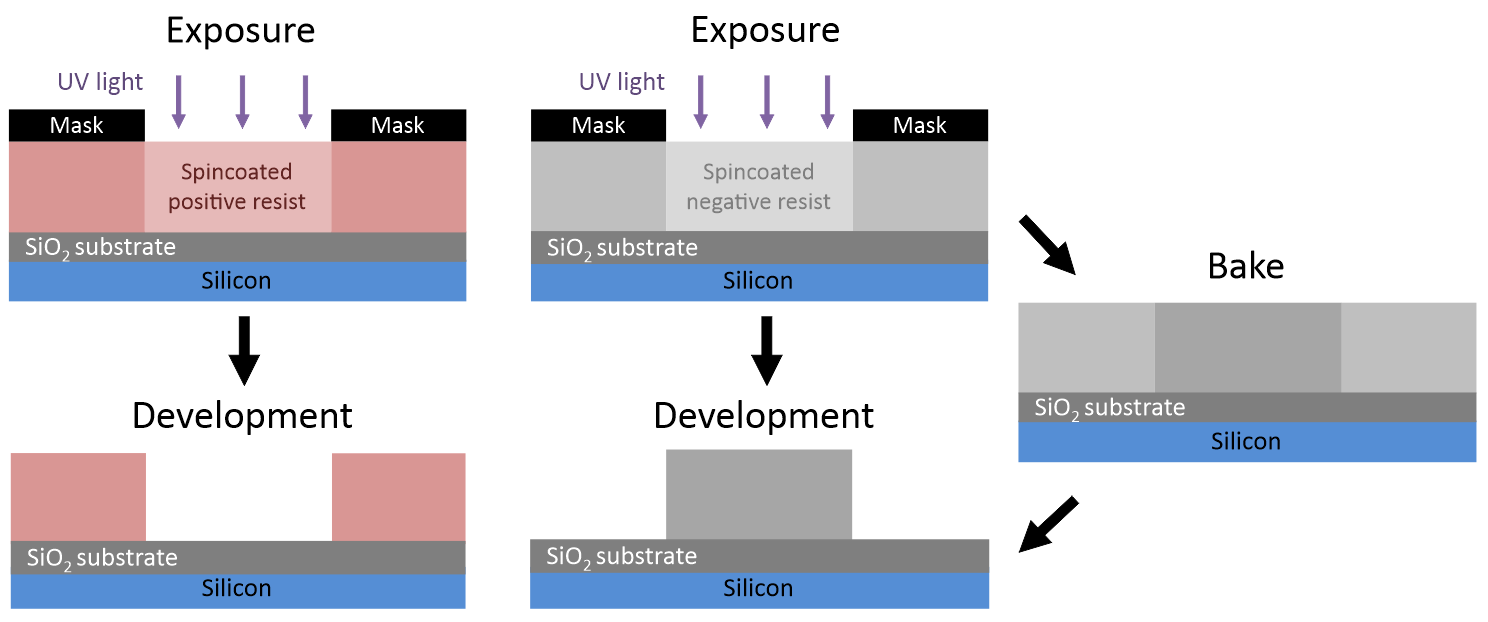
\includegraphics{figures/ch4/positive-negative-photolithography.png}

}

\caption{\label{fig-photolithography-types}A side-view comparison of
generic photolithography processes for positive and negative resists in
the ideal case. Photolithography with a positive resist requires a
single softbake step before exposure, while for negative resists a
second baking step is required after exposure (Thicknesses shown not to
scale).}

\end{figure}

This section details some of the standard photolithography procedures
used in the quarter wafer processing detailed in
Section~\ref{sec-qw-processing}. Photoresists, also referred to here as
`resists', are UV light-sensitive polymeric resins used for
photolithography. `Positive' resists are made soluble in alkalines by UV
light exposure, meaning exposed areas are removed in the development
process. Conversely, `negative' resists are cross-linked by exposure and
a post-exposure bake step. The unexposed areas of the negative resist
are then removed in the development process \autocite{Microchemicals}.
Both positive and negative resists are used in this thesis. The
processes for each type of resist are shown in
Figure~\ref{fig-photolithography-types}. The specific photoresist
selected for photolithography depends on the specific use case. The
types used in this thesis are positive and negative AZ\(^\circledR\)
photoresists (AZ\(^\circledR\) 1518, Microchemicals GmbH;
AZ\(^\circledR\) nLOF 2020, Microchemicals GmbH) and SU8 (SU8-2150,
Kayaku Advanced Materials, formerly Microchem). The AZ\(^\circledR\)
resists used have a minimum film thickness of
\(1.5\textrm{ } \textrm{µm}\) \autocite{Microchemicals}, while the
SU8-2150 has a minimum film thickness of \(0.5\textrm{ } \textrm{µm}\)
\autocite{Kayaku}.

\begin{figure}

\begin{minipage}[t]{0.03\linewidth}

{\centering 

\raisebox{-\height}{


\includegraphics{figures/(a).png}

}

}

\end{minipage}%
%
\begin{minipage}[t]{0.01\linewidth}

{\centering 

~

}

\end{minipage}%
%
\begin{minipage}[t]{0.45\linewidth}

{\centering 

\raisebox{-\height}{

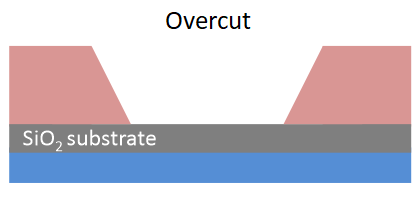
\includegraphics{figures/ch4/overcut-profile.png}

}

}

\end{minipage}%
%
\begin{minipage}[t]{0.01\linewidth}

{\centering 

~

}

\end{minipage}%
%
\begin{minipage}[t]{0.03\linewidth}

{\centering 

\raisebox{-\height}{

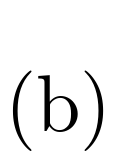
\includegraphics{figures/(b).png}

}

}

\end{minipage}%
%
\begin{minipage}[t]{0.01\linewidth}

{\centering 

~

}

\end{minipage}%
%
\begin{minipage}[t]{0.45\linewidth}

{\centering 

\raisebox{-\height}{

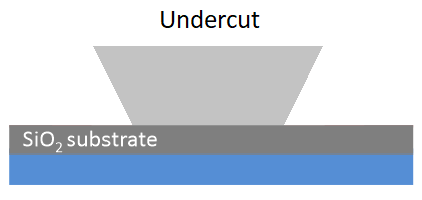
\includegraphics{figures/ch4/undercut-profile.png}

}

}

\end{minipage}%
%
\begin{minipage}[t]{0.01\linewidth}

{\centering 

~

}

\end{minipage}%

\caption{\label{fig-photolithography-profiles}The overcut profile of a
positive resist pattern is shown in (a). The undercut profile in (b) is
ideal for thin-film metal deposition and subsequent patterned removal,
known as ``lift-off''. Each profile has had the central region of the
substrate exposed to UV light prior to development.}

\end{figure}

Positive resists which have not been thermally crosslinked will soften
at higher temperatures (\(\gtrsim\) 100°C for AZ\(^\circledR\) 1518),
leading to a rounded profile. This is not the case for negative resists,
which are more thermally stable \autocite{Microchemicals}. Each resist
therefore has a different cross-section profile, as shown in
Figure~\ref{fig-photolithography-profiles}. If metal deposition is
performed on a positive resist, some metal can collect on the
outwardly-sloped sidewalls of the resist which forms significant spikes
on the edges of the deposited metal upon lift-off. The outwardly-sloped
or `overcut' resist profile is illustrated in
Figure~\ref{fig-photolithography-profiles} (a). On the other hand, metal
cannot collect on top of the inwardly-sloped negative profile sidewalls,
which avoids the formation of large edge spikes. The inwardly-sloped or
`undercut' profile is shown in
Figure~\ref{fig-photolithography-profiles} (b). Therefore, the negative
resist profile is more suited to metal or metal oxide deposition and
lift-off processes, though the process is more sensitive to human error
due to requiring more processing steps than positive resist
\autocite{Microchemicals}. Finally, when it is suitably processed, SU8
is considered to be more stable and biocompatible than other
photoresists \autocite{Albarghouthi2022}. It is especially biocompatible
when chemically modified via processes such as isopropanol sonication
and O\(_2\) plasma treatment \autocite{Chen2021}.

All photolithographic exposure was performed using a Karl Suss MJB3
Contact Aligner with a USHIO super-high pressure 350 W mercury lamp
(USH-350DS, Japan). When performing photolithography, the intensity
reading from the aligner was \(20.8-24.2\) mW/cm\(^2\) (Note however
that an external photometer reading at 400 nm found an intensity output
of 17.2 mW/cm\(^2\) when the aligner read 21.0 mW/cm\(^2\)). In general,
photolithography procedures should be performed under yellow lighting,
as light wavelengths from \(320-450\) nm can promote reactions in the
photoresist used and lead to a decline in photolithography quality.
Aging of photoresist over time can also significantly affect the
photolithography process, and therefore all processes should be
re-optimised regularly over time to give the desired result
\autocite{Microchemicals}. The range in processing times for some steps
of the processes used here are largely due to the effects of aging on
the photoresist. The step-by-step processes for each resist are detailed
in the subsequent sections.

\hypertarget{azcircledr-1518-photoresist}{%
\subsection{\texorpdfstring{AZ\(^\circledR\) 1518
photoresist}{AZ\^{}\textbackslash circledR 1518 photoresist}}\label{azcircledr-1518-photoresist}}

\begin{enumerate}
\def\labelenumi{\arabic{enumi}.}
\item
  Spincoat at a final speed of 4000 rotations per minute (rpm) for 1
  minute, with an initial acceleration of 500 rpm/s (notes: clean the
  substrate with acetone, isopropanol (IPA) and nitrogen before
  spincoating; use only the minimum amount of photoresist required to
  fully cover the wafer surface; avoid any gaps or bubbles in the
  photoresist).
\item
  Softbake \(2-4\) minutes at 95°C on the hotplate (2 min for individual
  devices, 4 min for a quarter wafer)
\item
  Mask expose for \(10-12\) s (note: clean mask with acetone/IPA and
  N\(_2\) dry before use)
\item
  Develop with 3 parts AZ\(^\circledR\) 326 (2.38 \% TMAH metal-ion free
  developer, Microchemicals GmbH) in 1 part deionised (DI) water for
  \(30-45\) s (note: rinse for \(10-15\) s in one development solution,
  then perform the rest of the development in clean developer for a
  cleaner profile; lightly agitate the solution throughout the
  development process)
\item
  Rinse device for 30 s in DI water to remove excess developer, then dry
  under nitrogen
\end{enumerate}

\hypertarget{azcircledr-nlof-2020-photoresist}{%
\subsection{\texorpdfstring{AZ\(^\circledR\) nLOF 2020
photoresist}{AZ\^{}\textbackslash circledR nLOF 2020 photoresist}}\label{azcircledr-nlof-2020-photoresist}}

\begin{enumerate}
\def\labelenumi{\arabic{enumi}.}
\item
  Spincoat at final speed of 3000 rotations per minute (rpm) for 1
  minute, with an initial acceleration of 500 rpm/s (notes: clean the
  substrate with acetone, isopropanol (IPA) and nitrogen before
  spincoating; avoid any gaps or bubbles in the photoresist)
\item
  Softbake for precisely 60 s at 110°C on the hotplate
\item
  Mask expose for \(2.7-3\) s (note: clean mask with acetone/IPA and
  N\(_2\) dry before use)
\item
  Post-exposure bake for precisely 60 s at 110°C on the hotplate to
  cross-link exposed resist
\item
  Develop with 3 parts AZ\(^\circledR\) 326 in 1 part DI water for
  \(60-70\) s (note: rinse for 30 s in one development solution, then
  perform the rest of the development in clean developer for a cleaner
  profile; lightly agitate the solution throughout the development
  process)
\item
  Rinse device for 30 s in DI water to remove excess developer, then dry
  under nitrogen
\end{enumerate}

\hypertarget{su8-2150-photoresist}{%
\subsection{SU8-2150 photoresist}\label{su8-2150-photoresist}}

\begin{enumerate}
\def\labelenumi{\arabic{enumi}.}
\item
  SU8 was diluted in cyclopentanone until viscosity was low enough to
  spincoat on substrate and then sonicated at \(50^\circ\)C for \(3-4\)
  hours (Note: The dilution ratio used was \(\sim\) 1 part SU8 to 5
  parts cyclopentanone. However, the age of the SU8 may mean that
  significant evaporation had occurred prior to use, and the amount of
  SU8 actually present is underrepresented by this ratio)
\item
  Spincoat first with a final speed of 500 rpm (acceleration 500 rpm/s)
  for 10 seconds, followed by spincoating at 4000 rpm (acceleration 7500
  rpm/s) for 40 s.
\item
  Softbake for 10 minutes at 95°C on the hotplate
\item
  Mask expose for \(6-8\) s (note: clean mask with acetone/IPA and
  N\(_2\) dry before use)
\item
  Post-exposure bake for 10 minutes at 95°C on the hotplate to
  cross-link exposed resist
\item
  Develop with SU8 developer (Kayaku Advanced Materials, formerly
  Microchem) for \(10-15\) s, then clean in IPA for 30 s, repeat this
  step once then dry under nitrogen (note: lightly agitate the solution
  throughout the development process)
\end{enumerate}

\hypertarget{sec-qw-processing}{%
\section{Fabrication of Carbon Nanotube and Graphene Field-Effect
Transistors}\label{sec-qw-processing}}

\hypertarget{overview}{%
\subsection{Overview}\label{overview}}

\begin{figure}

{\centering 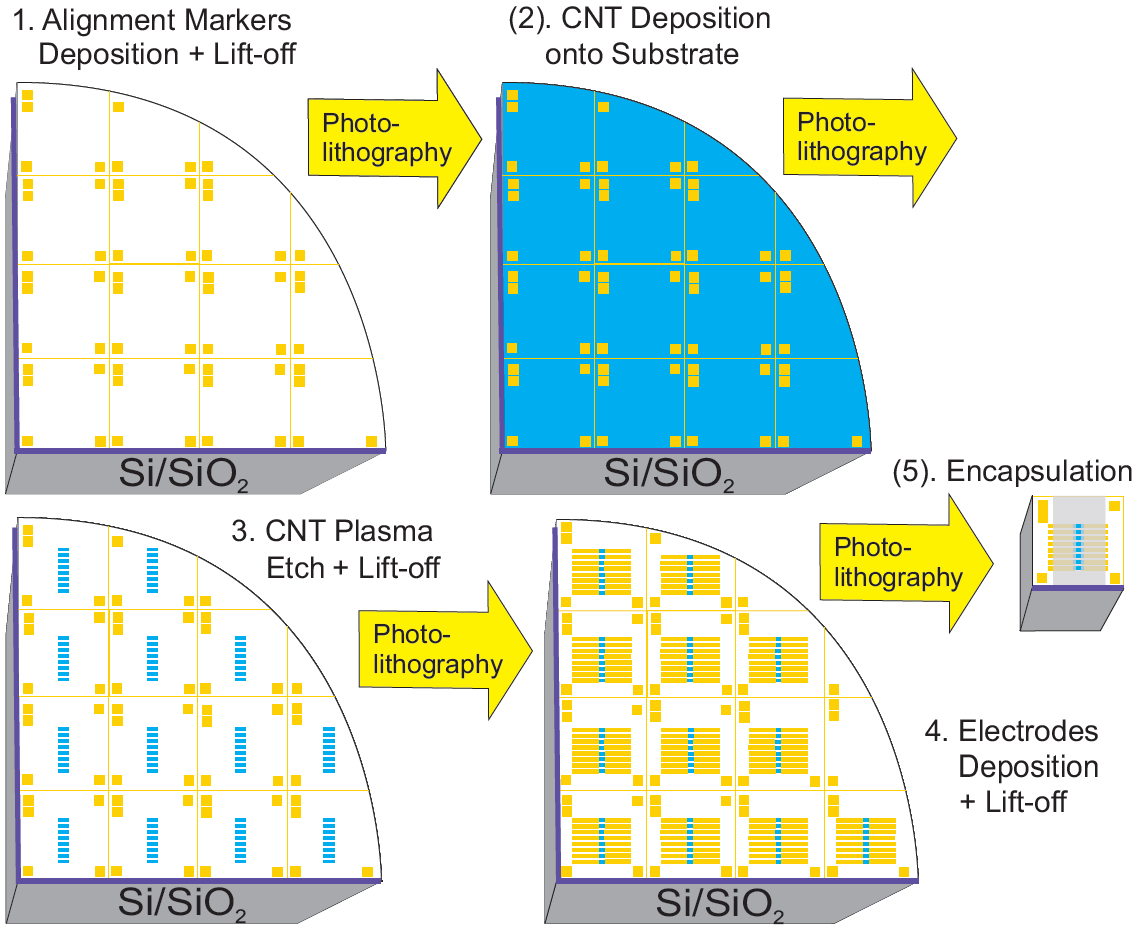
\includegraphics[width=0.9\textwidth,height=\textheight]{figures/ch4/photolithography-cycle.png}

}

\caption{\label{fig-qw-photolithography}The photolithographic processes
used for fabrication of both carbon nanotube and graphene devices
(graphene devices were fabricated individually for every step. Step 2 is
passed over for graphene devices).}

\end{figure}

Photolithography was used to define eight channel regions on each device
and subsequently to define metal contacts for each of these channels. A
schematic demonstrating these photolithography processes on a quarter
wafer is shown in Figure~\ref{fig-qw-photolithography}. Masks for
photolithography were designed in-house using LayoutEditor CAD software
and patterned externally with a UV laser writer. Thermal evaporation was
used when depositing chromium (Cr-plated tungsten rods, Kurt J. Lesker)
and gold (Au wire, 99.99\%, Regal Castings Ltd.), while electron beam
evaporation was used when depositing titanium (Ti pieces, 99.99\%, Kurt
J. Lesker) and metal oxides (\emph{e.g.} Al\(_2\)O\(_3\) pieces,
99.99\%, Kurt J. Lesker). Metal and metal oxide deposition was performed
using an Angstrom Engineering Nexdep 200 Vacuum Deposition System.
Deposition thickness was monitored by a Inficon quartz piezoelectric
sensor and controlled using an Inficon Deposition Controller. Electron
beam power was provided by a Telemark TT-6 power supply. For metals, the
chamber was initially evacuated to a pressure \(5 \times 10^{-6}\)
mTorr, while for metal oxides the chamber was initially evacuated to a
pressure of \(1 \times 10^{-5}\) mTorr. After evaporation, the chamber
was cooled and vented with nitrogen.

Carbon nanotube network field-effect transistors were fabricated using
4-inch \(p\)-type (B-doped) silicon wafers with either a 100 nm or 300
nm SiO\(_2\) layer (WaferPro LLC) as the substrate. Devices intended for
backgated measurements were fabricated with a 100 nm SiO\(_2\) layer.
Before photolithographic processing, the wafers were spin-coated with
AZ\(^\circledR\) 1518 photoresist, placed photoresist-side down onto a
cleanroom wipe, fixed in place using vacuum suction, then cleaved into
quarters using a diamond-tipped scribe tool. For fabrication performed
before Jun 2023, the protective photoresist layer was then removed by
soaking the quarter-wafers in acetone for 15 minutes, then rinsed with
isopropyl alcohol (IPA) and dried with N\(_2\) gas. However, for
complete removal of photoresist, it was necessary to flood expose the
wafer with the Karl Suss Aligner for 1 min and then place it in
AZ\(^\circledR\) 326 developer for 3 min, as discussed further in
\textbf{?@sec-photoresist-contamination}.

Graphene field-effect transistors were fabricated using 300 nm
SiO\(_2\)/\(p\)-type Si substrates covered with a monolayer of
mechanically transferred CVD graphene (Advanced Chemical Supplier). This
substrate was cleaved into equal-sized square chips before
photolithography, with side length between \(11.6-11.7\) mm, subject to
variability in wafer size. The same cleaving process outlined in
Section~\ref{sec-dep-carbon-nanotubes} was used for cleaving the chips,
but the photoresist was not rinsed off after cleaving. Devices were
exposed to a brief burst of N\(_2\) gas to remove any dust from the
cleaving process from the surface of devices. When not being used in
photolithography, graphene-based devices were stored in a vacuum
desiccator to prevent the quality of the graphene deteriorating with
exposure to air over time. The limited adhesion of graphene to the wafer
meant that photolithographic processing had to be performed particularly
carefully when fabricating graphene devices.

\begin{figure}

\begin{minipage}[t]{0.03\linewidth}

{\centering 

\raisebox{-\height}{


\includegraphics{figures/(a).png}

}

}

\end{minipage}%
%
\begin{minipage}[t]{0.01\linewidth}

{\centering 

~

}

\end{minipage}%
%
\begin{minipage}[t]{0.45\linewidth}

{\centering 

\raisebox{-\height}{

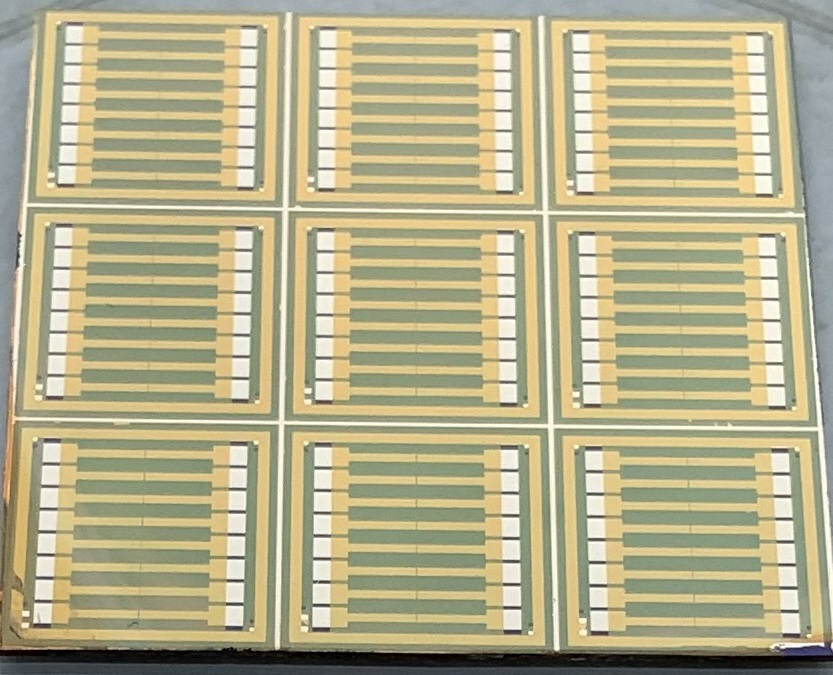
\includegraphics{figures/ch4/IMG_0845.png}

}

}

\end{minipage}%
%
\begin{minipage}[t]{0.01\linewidth}

{\centering 

~

}

\end{minipage}%
%
\begin{minipage}[t]{0.03\linewidth}

{\centering 

\raisebox{-\height}{

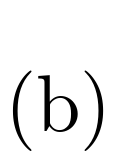
\includegraphics{figures/(b).png}

}

}

\end{minipage}%
%
\begin{minipage}[t]{0.01\linewidth}

{\centering 

~

}

\end{minipage}%
%
\begin{minipage}[t]{0.45\linewidth}

{\centering 

\raisebox{-\height}{

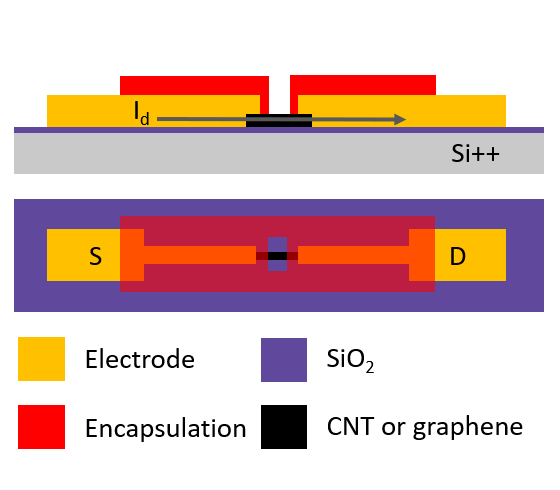
\includegraphics{figures/ch4/fet-schematic.png}

}

}

\end{minipage}%
%
\begin{minipage}[t]{0.01\linewidth}

{\centering 

~

}

\end{minipage}%

\caption{\label{fig-field-effect-transistor}A finished quarter-wafer
with the unusable edges cleaved off is shown in (a). Note the double
alignment markers feature in the bottom left corner of each device in
(a), indicating channel 1 `CH1'. The component parts of the field-effect
transistor are labelled on device cross-section and channel top view
schematics in (b).}

\end{figure}

From Jul 2023 onwards, after each photolithography step using negative
resist, quarter wafers/chips were placed in AZ\(^\circledR\) 326 or SU8
developer (depending on the type of resist) for 3 min to ensure complete
removal of photoresist residue. For each step with positive resist, the
same procedure was performed but with a flood exposure with UV light for
1 min before being placed in developer. The exception to this rule was
for devices with an aluminium oxide layer present. Tetramethylammonium
hydroxide (TMAH), the active ingredient of AZ\(^\circledR\) 326, etches
through aluminium oxide and causes electrical shorts through the
dielectric layer \autocite{Oh2011,Ali2021}. A further discussion showing
the results of this process is given in
\textbf{?@sec-photoresist-contamination}.
Figure~\ref{fig-field-effect-transistor} (a) shows a completed
quarter-wafer of carbon nanotube field-effect transistors, where partial
(unusable) devices at the edges of the wafer have been cleaved off so
that only a square of nine devices remains.
Figure~\ref{fig-field-effect-transistor} (b) shows cross-section and top
view schematics of the completed device with the component parts
labelled.

\hypertarget{sec-align}{%
\subsection{Alignment Markers}\label{sec-align}}

Metal alignment markers were deposited in order to accurately align the
device channels with device electrodes in subsequent photolithography
steps. These alignment markers were asymmetric to indicate the
orientation of the device for subsequent photolithography steps and
electrical characterisation. In later discussion, channel 1 is defined
as the channel placed closest to the large double square alignment
marker feature. For carbon nanotube quarter wafers, alignment markers
were deposited either directly before or after carbon nanotube
deposition (see Section~\ref{sec-dep-carbon-nanotubes} for discussion).
For graphene devices, alignment markers were deposited directly after
cleaving using the protective photoresist layer spincoated prior to
cleaving. AZ\(^\circledR\) 1518 was used for alignment marker
photolithography.

Adhesion layers are required to stick metals such as gold and platinum
to silicon dioxide. Chromium and titanium are the most common adhesion
metals, but palladium and nickel have also been used
successfully\autocite{Guarnieri2014,Shkodra2021}. For carbon nanotube
devices made before Jun 2022, chromium was used as an adhesive layer for
gold, while for all graphene devices and carbon nanotube devices made
after Jun 2022, titanium was used as the adhesive layer. Metal layer
thickness values quoted here are as stated on the Inficon controller.
These values are strictly nominal and must be corroborated, which was
done here using a Dektat profiler. For chromium/gold depositions, 10 nm
of chromium was deposited followed by a 100 nm Au layer. For
titanium/gold depositions, \(10-20\) nm of titanium was deposited
followed by a 50 nm Au layer. Devices were then soaked in acetone for at
least 2 hours for photoresist lift-off, washed in IPA and dried with
nitrogen. The use of titanium gave rise to a cleaner lift-off and
improved gold adhesion. Using a relatively thin gold layer (50 nm
nominal instead of 100 nm) also improved lift-off quality. Dektat
profiler measurements of combined metal layer thicknesses after lift-off
are described in Section~\ref{sec-electrodes}.

\hypertarget{sec-dep-carbon-nanotubes}{%
\subsection{Deposition of Carbon
Nanotubes}\label{sec-dep-carbon-nanotubes}}

Carbon nanotubes were deposited before the alignment markers
photolithography step on all wafers fabricated between Aug 2021 \(-\)
Feb 2023, while devices fabricated before Aug 2021 and after Feb 2023
had the alignment markers photolithography step performed before the
deposition of carbon nanotubes. The process order was first switched in
Aug 2021 as this order led to faster processing times. However, the
order was switched back in Feb 2023 to minimise the exposure of carbon
nanotubes to photolithographic chemical processes. The original,
solvent-based deposition process for the carbon nanotube network is as
follows. 10 mg of 2-mercaptopyridine (99\%, Sigma-Aldrich) was dissolved
in 1 mL ethanol by sonication until clear. Quarter wafers were sonicated
in acetone for 3 min, then exposed to O\(_2\) plasma at 100 W for at
least 2 min in a small plasma cleaner (Plasma Etch, Inc., PE-50 Compact
Benchtop Plasma Cleaning System) or reactive ion etcher (Oxford
Instruments, Plasmalab\(^\circledR\) 80 Plus) under 300 mTorr pressure.
The cleaned SiO\(_2\)/Si surface was then coated with 2-mercaptopyridine
for 10 minutes, rinsed with ethanol to remove residual
\(2\)-mercaptopyridine, and then nitrogen dried.

Meanwhile, 5 µg of 99\% semiconducting carbon nanotube bucky paper
(NanoIntegris, IsoNanotubes S-99) was dispersed in 10 mL of anhydrous
1,2-dichlorobenzene (DCB, Sigma Aldrich) by ultrasonication until no
particles were visible to the naked eye. During this time, the
ultrasonic bath temperature was kept between 20-30°C or the buckypaper
would not disperse successfully. The substrates were then placed into a
dish with CNT-DCB suspension and left covered for 1 hour, dipped into
ethanol for 10 min to remove residual solvent and any unattached carbon
nanotube bundles, and then dried with nitrogen. Devices fabricated using
films deposited in this manner are referred to in this thesis as
`solvent-deposited' networks.

\hypertarget{surfactant-based}{%
\subsubsection*{Surfactant-Based}\label{surfactant-based}}
\addcontentsline{toc}{subsubsection}{Surfactant-Based}

Two different approaches were used to attach the surfactant-dispersed
carbon nanotubes (CNTs) to the substrate surface. The first approach was
a simple drop-casting method, while the second was performed in the
presence of steam (`steam-assisted'). In both approaches, the quarter
wafers were first rinsed with ultrapure deionised water (DI water),
acetone and IPA. Next, they were placed into a small plasma cleaner
(Plasma Etch, Inc, PE-50 Compact Benchtop Plasma Cleaning System) or
reactive ion etcher (Oxford Instruments, Plasmalab 80 Plus) and exposed
to O\(_2\) plasma at 100 W for at least 2 min under 300 mTorr pressure
to make the surface hydrophilic. 1 mL of poly-\(L\)-lysine (PLL) was
immediately deposited onto each quarter wafer and left for 5 minutes.
The quarter wafers were then rinsed for 30 s with DI water and dried
with N\(_2\) gas. The presence of the PLL on the plasma cleaned surface
strengthens the surface adhesion of semiconducting single carbon
nanotubes after the surfactant dispersion has been dropcast onto the
substrate.

For carbon nanotube network films deposited in surfactant without steam
present, 2 mL of IsoNanotubes-S 90\% or 99\% dispersion (NanoIntegris)
was decanted into a small bottle and sonicated for 5 s to break up
bundles of CNTs\footnote{The composition of the surfactant used in the
  dispersion is proprietary to NanoIntegris.}. An even spread of 400 µL
carbon nanotube dispersion was placed in the centre of the
PLL-functionalised quarter wafer, covered with a glass dish and left for
10 minutes. The dispersion was then rinsed off with DI water and IPA,
and the quarter wafer was dried with N\(_2\) gas. Next, the quarter
wafer was annealed in a vacuum oven at 150°C for 1 hour to remove
residual surfactant. This method would often lead to an inhomogeneous
spread of CNTs across the quarter wafer surface, detailed further in
section \textbf{?@sec-cnt-deposition-effects}.

\begin{figure}

\begin{minipage}[t]{0.03\linewidth}

{\centering 

\raisebox{-\height}{


\includegraphics{figures/(a).png}

}

}

\end{minipage}%
%
\begin{minipage}[t]{0.01\linewidth}

{\centering 

~

}

\end{minipage}%
%
\begin{minipage}[t]{0.45\linewidth}

{\centering 

\raisebox{-\height}{

\includegraphics{figures/ch4/steaming-method-top.png}

}

}

\end{minipage}%
%
\begin{minipage}[t]{0.01\linewidth}

{\centering 

~

}

\end{minipage}%
%
\begin{minipage}[t]{0.03\linewidth}

{\centering 

\raisebox{-\height}{

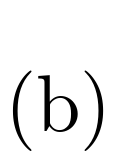
\includegraphics{figures/(b).png}

}

}

\end{minipage}%
%
\begin{minipage}[t]{0.01\linewidth}

{\centering 

~

}

\end{minipage}%
%
\begin{minipage}[t]{0.45\linewidth}

{\centering 

\raisebox{-\height}{

\includegraphics{figures/ch4/steaming-method-side.png}

}

}

\end{minipage}%
%
\begin{minipage}[t]{0.01\linewidth}

{\centering 

~

}

\end{minipage}%

\caption{\label{fig-steaming-method}Top view (a) and side view (b) of
the steam-assisted method setup, with and without the glass steam cover
above the quarter wafer.}

\end{figure}

For carbon nanotube network films deposited in surfactant in the
presence of steam, 2 mL of IsoNanotubes-S 90\% or 99\% dispersion
(NanoIntegris) was decanted into a small bottle and burst-sonicated once
to break up bundles of carbon nanotubes. Subsequently, 75 mL of 95°C
water was placed into a glass dish on a hotplate held at 95°C. After
this, the PLL-functionalised quarter wafer was placed in the centre of
an insulating surface on the same hotplate. The carbon nanotube
dispersion was carefully spread across the surface of the wafer without
spilling any over the wafer edges. The wafer on the insulating surface
and glass dish were then left under the same glass dish for 2 minutes to
expose the wafer to steam from the glass dish. The use of an insulating
surface meant that the wafer and dispersion were not heated from below
while exposed to steam. The steam-assisted deposition setup is shown in
Figure~\ref{fig-steaming-method}, where (a) shows the top and (b) shows
the side view of the process.

The carbon nanotube dispersion was then rinsed off the wafer with DI
water, ethanol, acetone and IPA, and then the quarter wafer was dried
with N\(_2\) gas. As in the original method, the quarter wafer was then
annealed in a vacuum oven at 150°C for 1 hour to remove residual
surfactant. This method gave an even spread of CNTs across the quarter
wafer surface, leading to a greater consistency in performance between
devices. Further details can be found in
\textbf{?@sec-cnt-deposition-effects}. Devices fabricated using films
deposited in this manner are sometimes referred to here as
``steam-deposited'' or ``steam-assisted surfactant-deposited'' networks
(rather than simply ``surfactant-deposited'', to avoid confusion with
the steam-free method).

\hypertarget{channel-etching}{%
\subsection{Channel Etching}\label{channel-etching}}

\begin{figure}

\begin{minipage}[t]{0.03\linewidth}

{\centering 

\raisebox{-\height}{


\includegraphics{figures/(a).png}

}

}

\end{minipage}%
%
\begin{minipage}[t]{0.01\linewidth}

{\centering 

~

}

\end{minipage}%
%
\begin{minipage}[t]{0.45\linewidth}

{\centering 

\raisebox{-\height}{

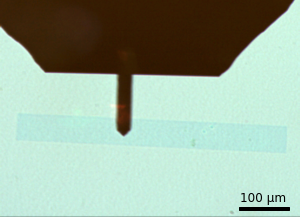
\includegraphics{figures/ch4/channel-area.png}

}

}

\end{minipage}%
%
\begin{minipage}[t]{0.01\linewidth}

{\centering 

~

}

\end{minipage}%
%
\begin{minipage}[t]{0.03\linewidth}

{\centering 

\raisebox{-\height}{

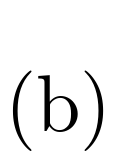
\includegraphics{figures/(b).png}

}

}

\end{minipage}%
%
\begin{minipage}[t]{0.01\linewidth}

{\centering 

~

}

\end{minipage}%
%
\begin{minipage}[t]{0.45\linewidth}

{\centering 

\raisebox{-\height}{

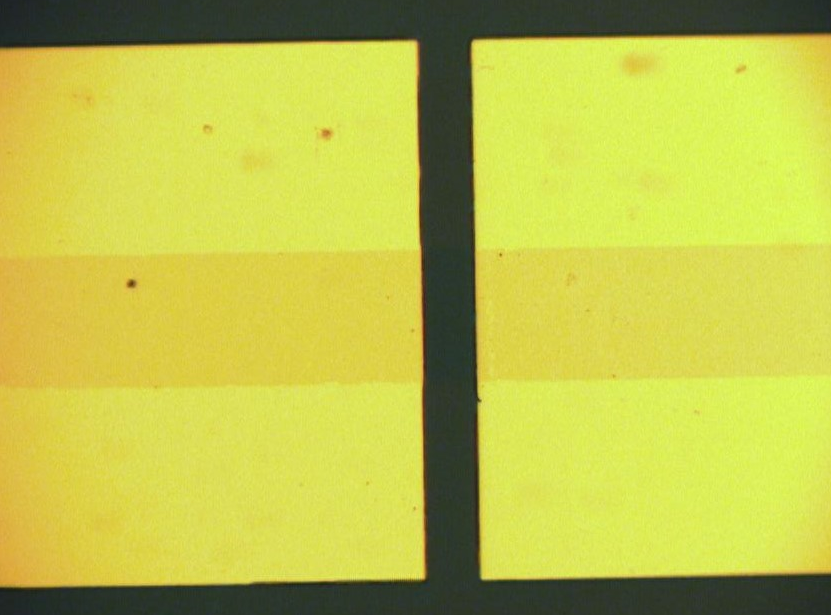
\includegraphics{figures/ch4/graphene-channel-electrodes.png}

}

}

\end{minipage}%
%
\begin{minipage}[t]{0.01\linewidth}

{\centering 

~

}

\end{minipage}%

\caption{\label{fig-microscope-graphene-channel}A graphene channel after
the plasma etch step is shown in (a), and (b) shows another graphene
channel after the metal electrode deposition and liftoff step.}

\end{figure}

Eight channel features, each 1000 µm in length and 100 µm in width with
a pitch of 1200 µm, were patterned using AZ\(^\circledR\) 1518
photolithography on each carbon nanotube or graphene-covered substrate.
Unwanted nanomaterial not covered with photoresist was then etched away
with 200 W oxygen plasma at 600 mTorr using a reactive ion etcher or RIE
(Plasmalab\(^\circledR\) 80 Plus, Oxford Instruments). The etch time was
3 minutes for carbon nanotube quarter wafers, and 1 minute for graphene
chips. The protective photoresist was then removed by soaking in acetone
for at least 5 minutes. The graphene channel feature after etching is
shown in Figure~\ref{fig-microscope-graphene-channel} (a).

\hypertarget{sec-electrodes}{%
\subsection{Source and Drain Electrodes}\label{sec-electrodes}}

The source and drain electrodes for each channel were patterned using
photolithography with either AZ\(^\circledR\) 1518 photoresist (pre-Mar
2023) or AZ\(^\circledR\) nLOF 2020 photoresist (post-Mar 2023). Before
metal deposition, the developed photoresist pattern was exposed to
O\(_2\) plasma at 50 W for up to 5 s or at 20 W for \(20-25\) s in a
PE-50 plasma cleaner (Plasma Etch, Inc.) to remove residual photoresist
on the developed regions and ensure a clean lift-off. After metal
deposition, wafers/devices were soaked in acetone for at least 2 hours
for photoresist lift-off, washed in IPA and dried with nitrogen. A
graphene channel feature after electrodes deposition is shown in
Figure~\ref{fig-microscope-graphene-channel} (b). As with the alignment
markers deposition (see Section~\ref{sec-align}), before Jun 2022
chromium was used for the gold adhesion layer, and after Jun 2022
titanium was used. A 20 nm nominal titanium thickness instead of 10 nm
nominal thickness was found to give better electrode adhesion, and
devices after Feb 2023 were made using this thicker adhesion layer. Good
electronic contact could be made with electrodes with a nominal gold
layer thickness of \(60-100\) nm, and a Au layer nominally 100 nm thick
was most commonly used.

\begin{figure}

\begin{minipage}[t]{0.03\linewidth}

{\centering 

\raisebox{-\height}{


\includegraphics{figures/(a).png}

}

}

\end{minipage}%
%
\begin{minipage}[t]{0.01\linewidth}

{\centering 

~

}

\end{minipage}%
%
\begin{minipage}[t]{0.45\linewidth}

{\centering 

\raisebox{-\height}{

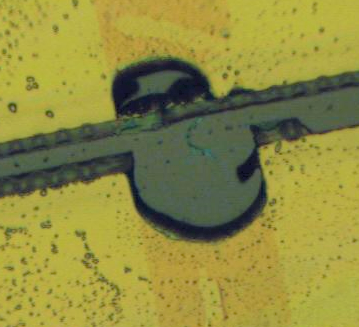
\includegraphics{figures/ch4/apr-21-dmso-damage.png}

}

}

\end{minipage}%
%
\begin{minipage}[t]{0.01\linewidth}

{\centering 

~

}

\end{minipage}%
%
\begin{minipage}[t]{0.03\linewidth}

{\centering 

\raisebox{-\height}{

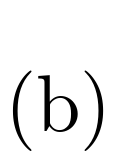
\includegraphics{figures/(b).png}

}

}

\end{minipage}%
%
\begin{minipage}[t]{0.01\linewidth}

{\centering 

~

}

\end{minipage}%
%
\begin{minipage}[t]{0.45\linewidth}

{\centering 

\raisebox{-\height}{

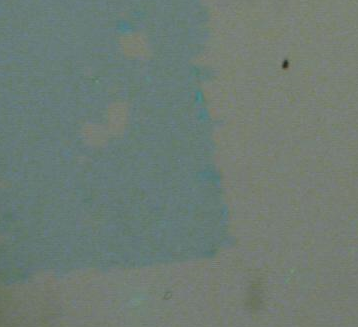
\includegraphics{figures/ch4/may-21-dmso-damage.png}

}

}

\end{minipage}%
%
\begin{minipage}[t]{0.01\linewidth}

{\centering 

~

}

\end{minipage}%

\caption{\label{fig-dmso-damage}Damage to the gold electrode in the
graphene channel region after dimethyl sulfoxide lift-off is shown in
(a), while (b) shows damage to a graphene film (blue-green region) after
dimethyl sulfoxide lift-off.}

\end{figure}

Dimethyl sulfoxide (DMSO) was sometimes used in electrodes lift-off
instead of acetone between Jul 2021 and Feb 2023 because of its
effectiveness as a photoresist stripping agent. However, it was
abandoned due to some indications it was unsuitable for the devices
being fabricated. Figure~\ref{fig-dmso-damage} (a) shows damage by the
DMSO to the gold electrodes, and Figure~\ref{fig-dmso-damage} (b) shows
graphene damaged during the DMSO lift-off. also as detailed in
\textbf{?@sec-cnt-deposition-effects}. It is possible that heat from the
electrodes deposition sometimes crosslinked residual photoresist on the
nanomaterial, and then during lift-off was removed together with any
attached nanomaterial by the DMSO. However, it is also possible that
prolonged exposure to DMSO alone was sufficient to detach nanomaterial
from the substrate. Therefore, acetone was the preferred agent for
lift-off despite being a less efficient stripping agent than DMSO.

\begin{figure}

\begin{minipage}[t]{0.03\linewidth}

{\centering 

\raisebox{-\height}{


\includegraphics{figures/(a).png}

}

}

\end{minipage}%
%
\begin{minipage}[t]{0.01\linewidth}

{\centering 

~

}

\end{minipage}%
%
\begin{minipage}[t]{0.45\linewidth}

{\centering 

\raisebox{-\height}{

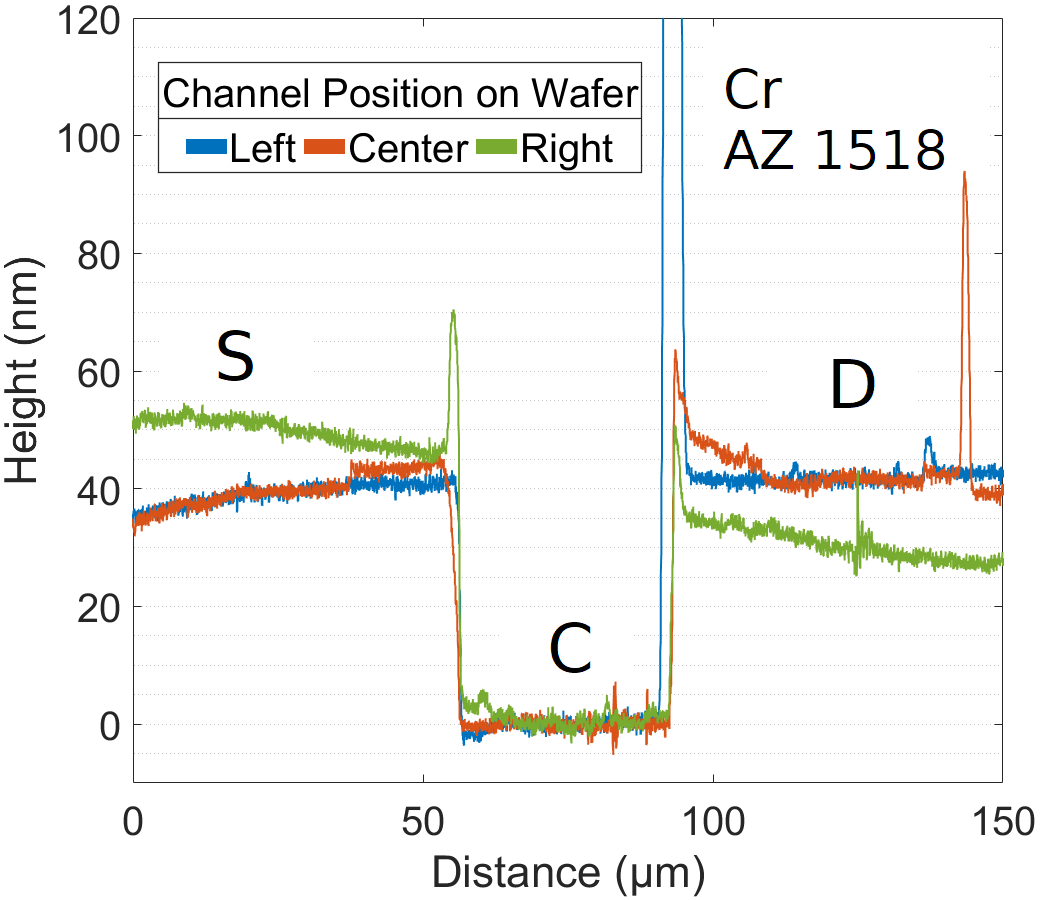
\includegraphics{figures/ch4/dektat_cr_electrodes_edit.png}

}

}

\end{minipage}%
%
\begin{minipage}[t]{0.01\linewidth}

{\centering 

~

}

\end{minipage}%
%
\begin{minipage}[t]{0.03\linewidth}

{\centering 

\raisebox{-\height}{

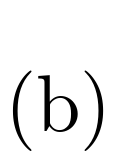
\includegraphics{figures/(b).png}

}

}

\end{minipage}%
%
\begin{minipage}[t]{0.01\linewidth}

{\centering 

~

}

\end{minipage}%
%
\begin{minipage}[t]{0.45\linewidth}

{\centering 

\raisebox{-\height}{

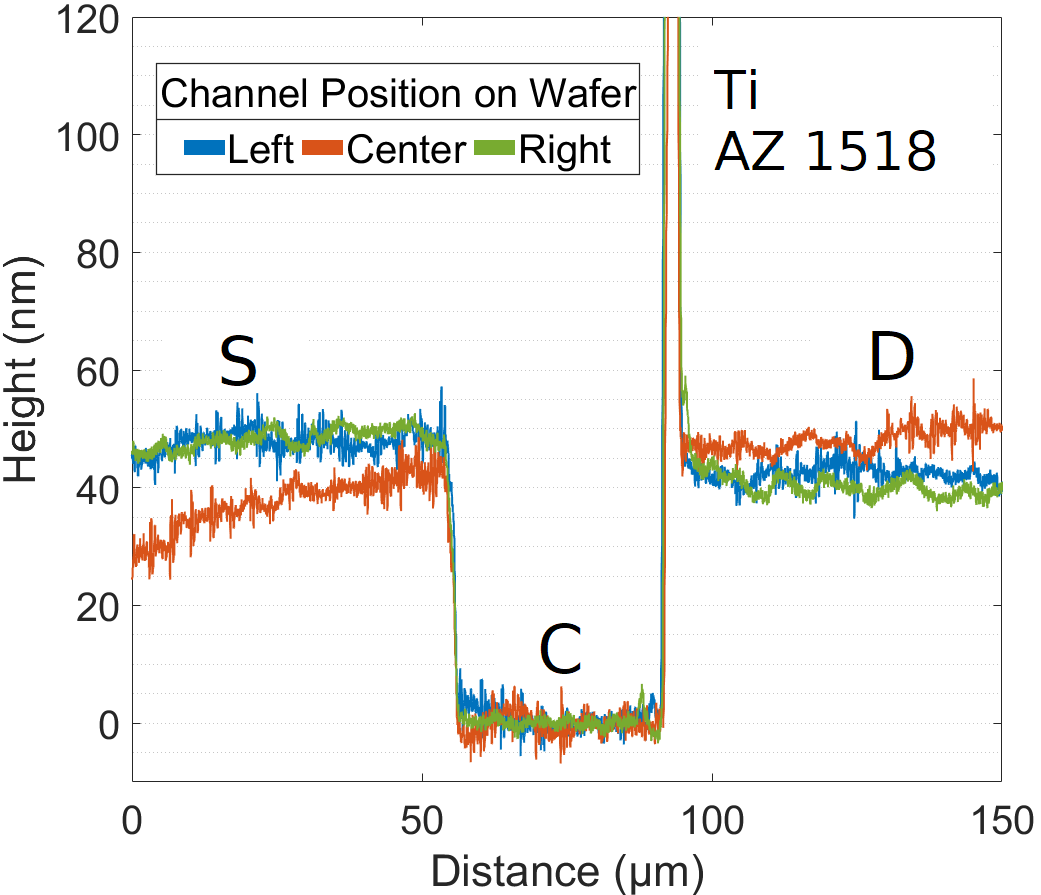
\includegraphics{figures/ch4/dektat_ti_electrodes_edit.png}

}

}

\end{minipage}%
%
\begin{minipage}[t]{0.01\linewidth}

{\centering 

~

}

\end{minipage}%
\newline
\begin{minipage}[t]{0.03\linewidth}

{\centering 

\raisebox{-\height}{


\includegraphics{figures/(c).png}

}

}

\end{minipage}%
%
\begin{minipage}[t]{0.01\linewidth}

{\centering 

~

}

\end{minipage}%
%
\begin{minipage}[t]{0.45\linewidth}

{\centering 

\raisebox{-\height}{

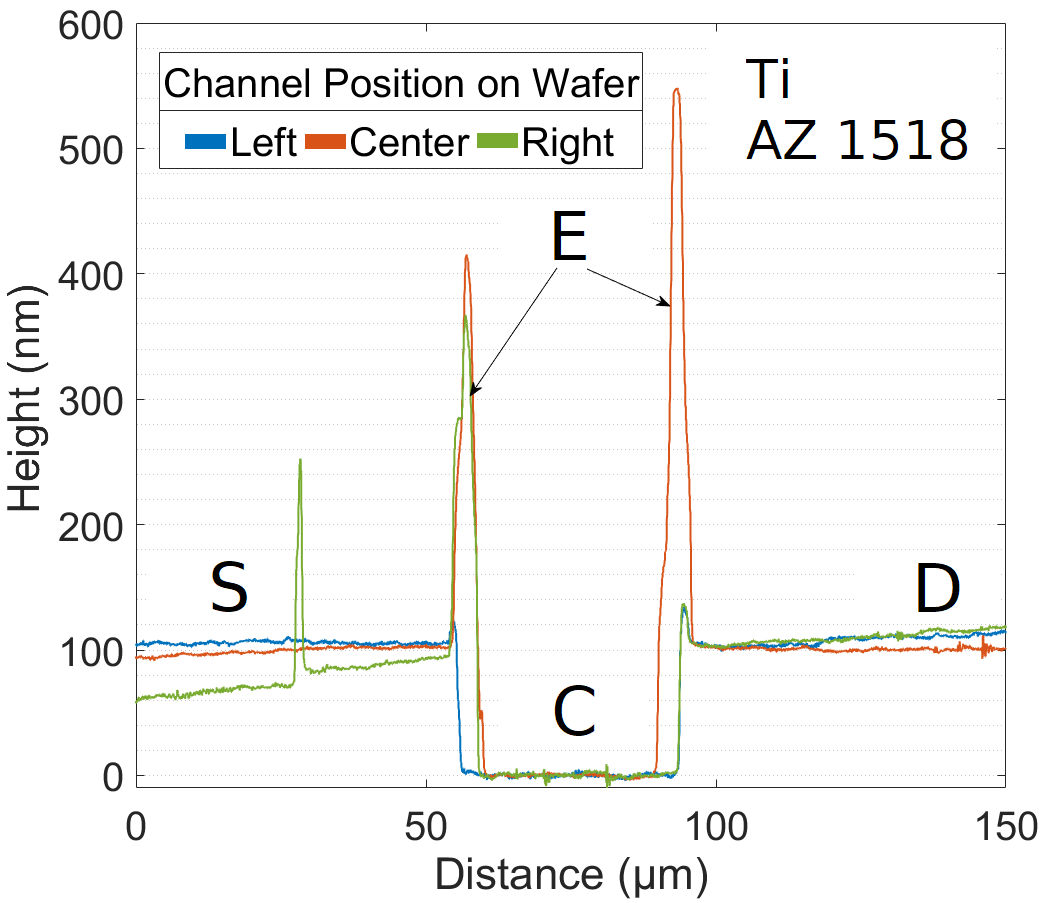
\includegraphics{figures/ch4/dektat_1518_electrode_profile_edit.png}

}

}

\end{minipage}%
%
\begin{minipage}[t]{0.01\linewidth}

{\centering 

~

}

\end{minipage}%
%
\begin{minipage}[t]{0.03\linewidth}

{\centering 

\raisebox{-\height}{

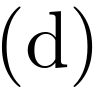
\includegraphics{figures/(d).png}

}

}

\end{minipage}%
%
\begin{minipage}[t]{0.01\linewidth}

{\centering 

~

}

\end{minipage}%
%
\begin{minipage}[t]{0.45\linewidth}

{\centering 

\raisebox{-\height}{

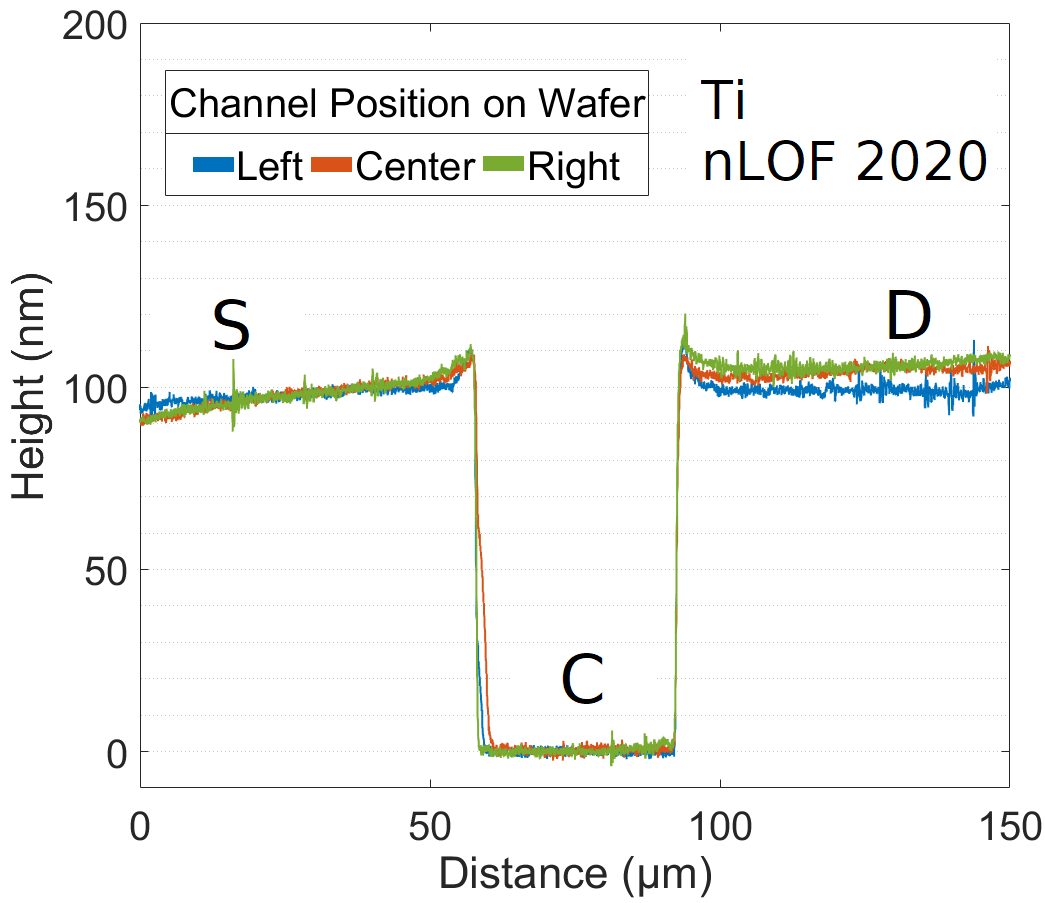
\includegraphics{figures/ch4/dektat_nlof_electrode_profile_edit.png}

}

}

\end{minipage}%
%
\begin{minipage}[t]{0.01\linewidth}

{\centering 

~

}

\end{minipage}%

\caption{\label{fig-electrodes-dektat}The Dektat height profile
measurements for source and drain electrodes taken at different
locations on four different quarter wafers are shown here. A 10 nm
adhesion layer and 100 nm Au layer were used for the wafers in (a) and
(b), with chromium as the adhesion layer for (a) and titanium for (b). A
20 nm titanium adhesion layer and 100 nm Au layer were used for both (c)
and (d). AZ\(^\circledR\) 1518 photolithography was used in (a)-(c),
while AZ\(^\circledR\) nLOF2020 was used in (d). S is source electrode,
D is drain electrode and C is the channel region. E indicates the edge
spikes or `cat ears' features.}

\end{figure}

Example height profiles of quarter wafer channels taken using a Veeco
Dektat 150 profiler are shown in Figure~\ref{fig-electrodes-dektat}.
AZ\(^\circledR\) 1518 photoresist was used in
Figure~\ref{fig-electrodes-dektat} (a) and
Figure~\ref{fig-electrodes-dektat} (b) for photolithographic patterning.
A 10 nm adhesion layer and 100 nm Au layer were used for each quarter
wafers to ensure a consistent comparison. From these figures, a Cr/Au
electrode height of \(42\pm1\) nm and a Ti/Au electrode height of
\(48\pm2\) nm were measured, slightly less than half the respective
heights stated on the Inficon Deposition Controller. Although using
AZ\(^\circledR\) nLOF 2020 photolithography involves more processing
steps, it gave rise to more cleanly-defined electrodes with a more
consistent height profile. Often electrode deposition using
AZ\(^\circledR\) 1518 photoresist would lead to sharp vertical spikes
along the edge of the electrode, as seen in
Figure~\ref{fig-electrodes-dektat} (c). These edge spikes or `cat ears'
can partially or fully protrude through thin encapsulation materials
such as SU8 and Al\(_2\)O\(_3\), leading to significant leakage currents
from the electrodes into the FET top gate. This effect is due to the
profile of positive resists being suboptimal for lift-off processes, as
discussed in Section~\ref{sec-photolithography}.

The height profile corresponding to a wafer with electrodes fabricated
using AZ\(^\circledR\) nLOF 2020 is shown in
Figure~\ref{fig-electrodes-dektat} (d). A 20 nm titanium adhesion layer
and 100 nm Au layer were used for both
Figure~\ref{fig-electrodes-dektat} (c) and
Figure~\ref{fig-electrodes-dektat} (d) to ensure a consistent
comparison, resulting in a measured electrode height of \(103\pm2\) nm
for both wafers. A comparison of these figures indicates that
AZ\(^\circledR\) nLOF 2020 photoresist has a more consistent electrode
height profile across the wafer surface than the wafer which used
AZ\(^\circledR\) 1518 resist. The measured edge features for the
AZ\(^\circledR\) 1518 resist electrodes vary in size from 20 nm to 450
nm above the bulk electrode surface, whereas the edge features for the
AZ\(^\circledR\) nLOF 2020 resist do not exceed 14 nm in height.

\hypertarget{sec-encapsulation}{%
\subsection{Encapsulation}\label{sec-encapsulation}}

Several different approaches were used for the encapsulation, or contact
protection, of devices. The encapsulation of graphene and
carbon-nanotube transistors for biosensing is essential to improve
transistor characteristics, passivate the electrodes and ensure only the
nanomaterial region is active during biosensing, as discussed in
\textbf{?@sec-biosensor-methods}. Before encapsulation photolithography
the carbon-nanotube network quarter wafers were cleaved into individual
11 mm \(\times\) 11 mm chips, using the cleaving process outlined in
Section~\ref{sec-dep-carbon-nanotubes}. Cleaving the devices at this
step ensured consistent thickness across photoresist encapsulated
devices, giving a less variable photolithographic pattern after UV
exposure and development.

\begin{figure}

\begin{minipage}[t]{0.03\linewidth}

{\centering 

\raisebox{-\height}{


\includegraphics{figures/(a).png}

}

}

\end{minipage}%
%
\begin{minipage}[t]{0.01\linewidth}

{\centering 

~

}

\end{minipage}%
%
\begin{minipage}[t]{0.45\linewidth}

{\centering 

\raisebox{-\height}{

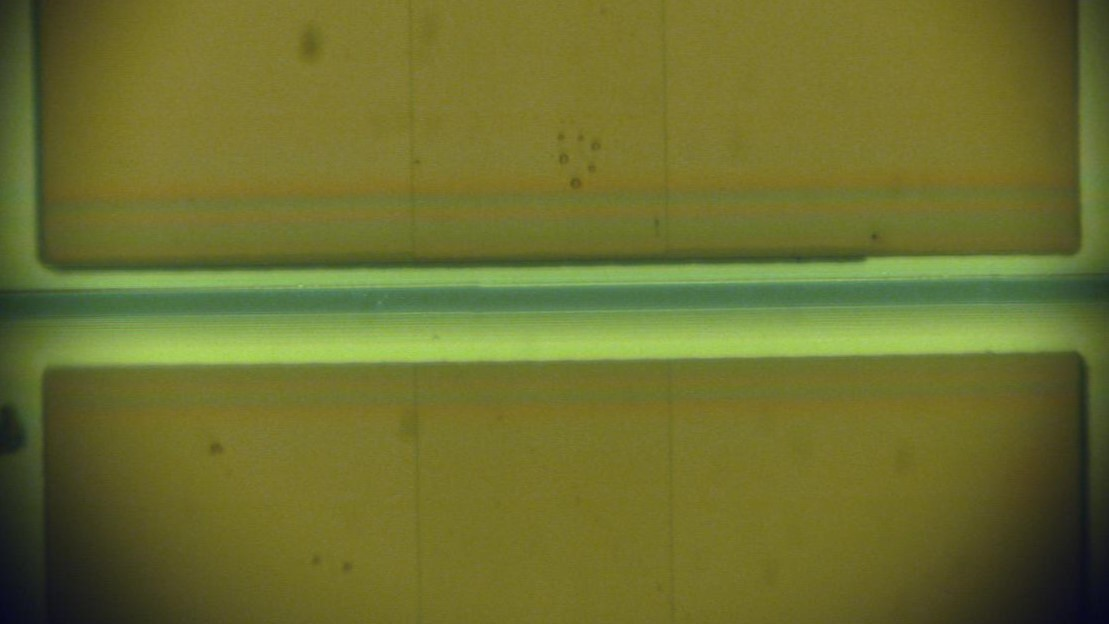
\includegraphics{figures/ch4/encapsulation_old.png}

}

}

\end{minipage}%
%
\begin{minipage}[t]{0.01\linewidth}

{\centering 

~

}

\end{minipage}%
%
\begin{minipage}[t]{0.03\linewidth}

{\centering 

\raisebox{-\height}{

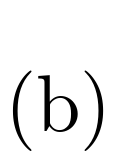
\includegraphics{figures/(b).png}

}

}

\end{minipage}%
%
\begin{minipage}[t]{0.01\linewidth}

{\centering 

~

}

\end{minipage}%
%
\begin{minipage}[t]{0.45\linewidth}

{\centering 

\raisebox{-\height}{

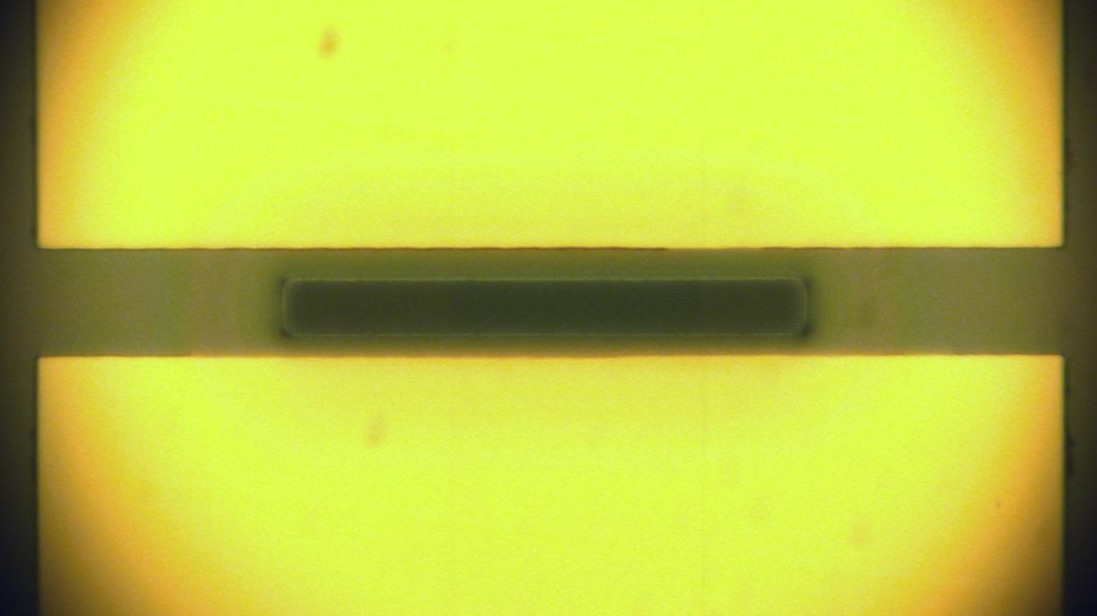
\includegraphics{figures/ch4/encapsulation_new.png}

}

}

\end{minipage}%
%
\begin{minipage}[t]{0.01\linewidth}

{\centering 

~

}

\end{minipage}%

\caption{\label{fig-microscope-encapsulation}A side-by-side microscope
comparison of hardbaked AZ\(^\circledR\) 1518 processed using the
pre-2023 mask, shown in (a), and the 2023 mask, shown in (b).}

\end{figure}

Two different photolithography masks were used for encapsulation
photolithography in this work, with different exposed areas of active
nanomaterial. The first mask was used for devices made before Jan 2023,
and was designed to leave a region of 500 µm \(\times\) 10 µm
unencapsulated for each channel. The second mask was used exclusively
after Jan 2023, and was designed to leave a region of 200 µm \(\times\)
20 µm unencapsulated for each channel. This change was made to double
the area of carbon nanotubes exposed to electrolyte while halving the
area of SiO\(_2\) dielectric exposed to electrolyte during aqueous
sensing. Figure~\ref{fig-microscope-encapsulation} (a) shows the
encapsulation pattern resulting from using the old mask for UV exposure,
while the encapsulation pattern resulting from using the new mask is
shown in Figure~\ref{fig-microscope-encapsulation} (b). The Dektat
profiles of three different devices encapsulated using the old mask as
used in Figure~\ref{fig-microscope-encapsulation} (a) are shown in
Figure~\ref{fig-microscope-encapsulation} (a) and
Figure~\ref{fig-microscope-encapsulation} (b) for AZ\(^\circledR\) 1518
and SU8 resist respectively, while AZ\(^\circledR\) 1518 and SU8
profiles encapsulated using the new mask as used in
Figure~\ref{fig-microscope-encapsulation} (b) are shown for in
Figure~\ref{fig-dektat-encapsulation} (c) and
Figure~\ref{fig-dektat-encapsulation} (d) respectively. The profiles
corresponding to the mask used after Jan 2023 clearly exhibit greater
device-to-device consistency, partly due to the mask requiring a greater
level of accuracy when aligning the encapsulation pattern with the
electrode channel. The larger feature size also means development time
has less of an impact on the quality of the encapsulation opening.

\begin{figure}

\begin{minipage}[t]{0.03\linewidth}

{\centering 

\raisebox{-\height}{


\includegraphics{figures/(a).png}

}

}

\end{minipage}%
%
\begin{minipage}[t]{0.01\linewidth}

{\centering 

~

}

\end{minipage}%
%
\begin{minipage}[t]{0.45\linewidth}

{\centering 

\raisebox{-\height}{

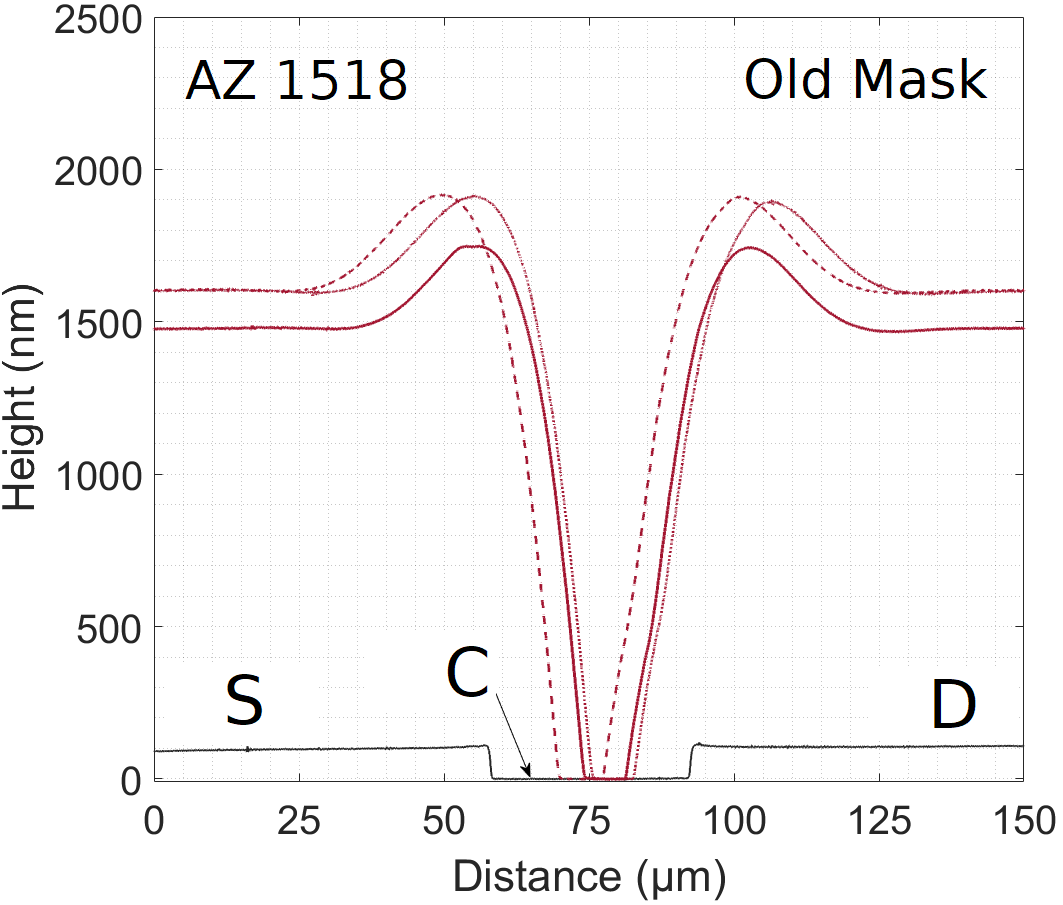
\includegraphics{figures/ch4/dektat_AZ1518_oldmask_edit.png}

}

}

\end{minipage}%
%
\begin{minipage}[t]{0.01\linewidth}

{\centering 

~

}

\end{minipage}%
%
\begin{minipage}[t]{0.03\linewidth}

{\centering 

\raisebox{-\height}{

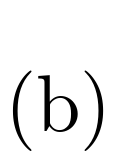
\includegraphics{figures/(b).png}

}

}

\end{minipage}%
%
\begin{minipage}[t]{0.01\linewidth}

{\centering 

~

}

\end{minipage}%
%
\begin{minipage}[t]{0.45\linewidth}

{\centering 

\raisebox{-\height}{

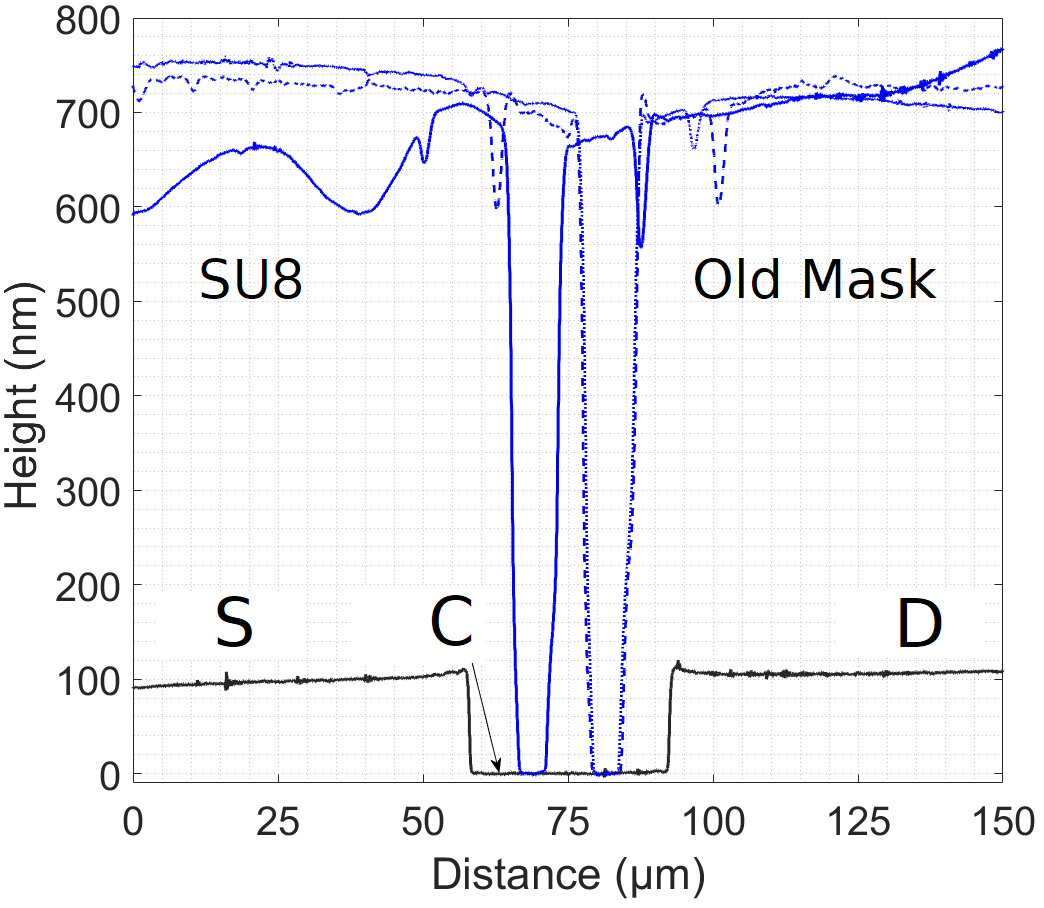
\includegraphics{figures/ch4/dektat_SU8_oldmask_edit.png}

}

}

\end{minipage}%
%
\begin{minipage}[t]{0.01\linewidth}

{\centering 

~

}

\end{minipage}%
\newline
\begin{minipage}[t]{0.03\linewidth}

{\centering 

\raisebox{-\height}{


\includegraphics{figures/(c).png}

}

}

\end{minipage}%
%
\begin{minipage}[t]{0.01\linewidth}

{\centering 

~

}

\end{minipage}%
%
\begin{minipage}[t]{0.45\linewidth}

{\centering 

\raisebox{-\height}{

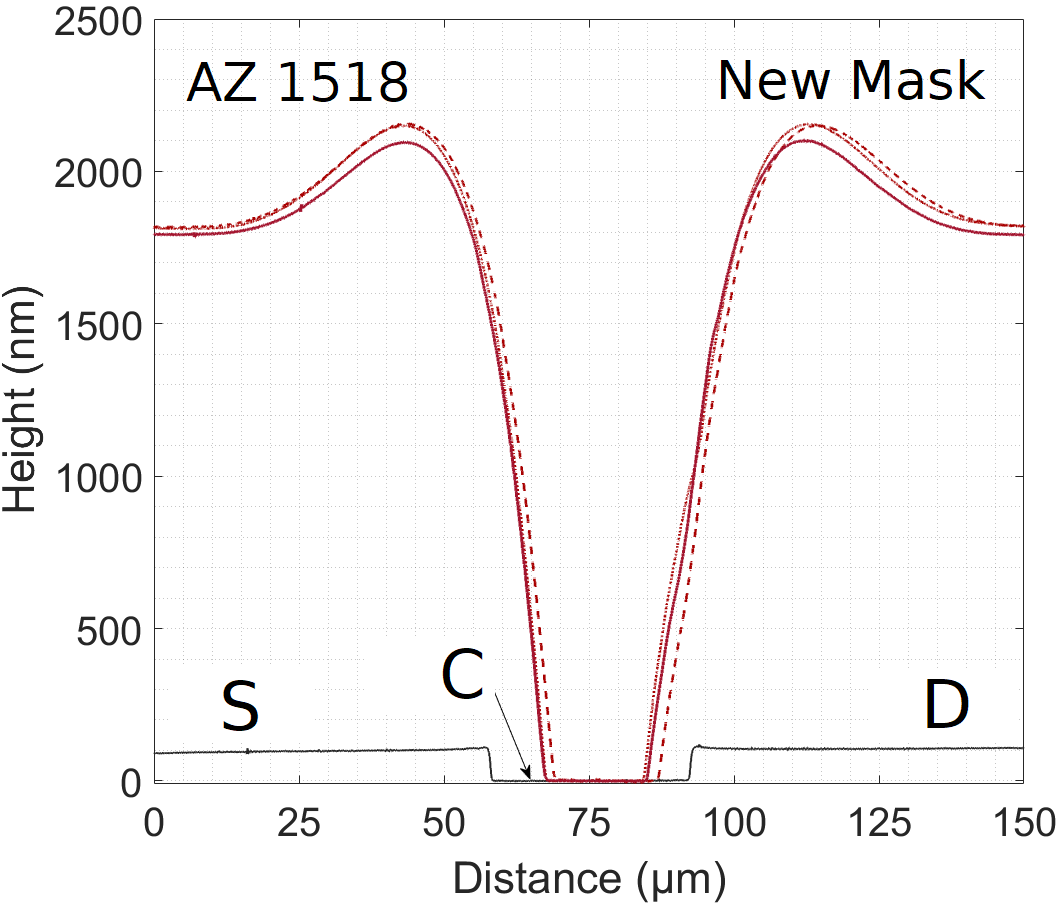
\includegraphics{figures/ch4/dektat_AZ1518_newmask_edit.png}

}

}

\end{minipage}%
%
\begin{minipage}[t]{0.01\linewidth}

{\centering 

~

}

\end{minipage}%
%
\begin{minipage}[t]{0.03\linewidth}

{\centering 

\raisebox{-\height}{

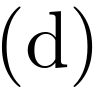
\includegraphics{figures/(d).png}

}

}

\end{minipage}%
%
\begin{minipage}[t]{0.01\linewidth}

{\centering 

~

}

\end{minipage}%
%
\begin{minipage}[t]{0.45\linewidth}

{\centering 

\raisebox{-\height}{

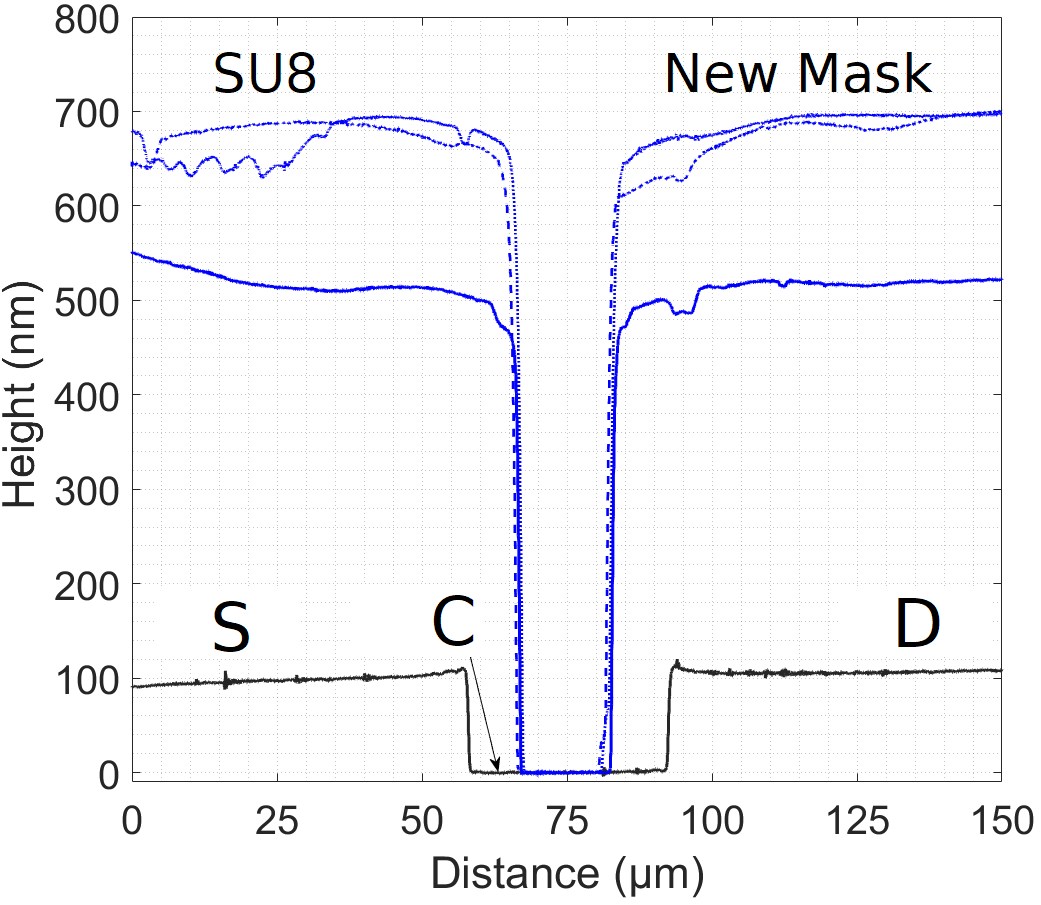
\includegraphics{figures/ch4/dektat_SU8_newmask_edit.png}

}

}

\end{minipage}%
%
\begin{minipage}[t]{0.01\linewidth}

{\centering 

~

}

\end{minipage}%

\caption{\label{fig-dektat-encapsulation}Dektat of carbon nanotube
devices after encapsulation photolithography using hardbaked
AZ\(^\circledR\) 1518 and SU8-2150, taken from three different devices.
(a) and (b) show photolithography performed with the old, pre-2023 mask,
using AZ\(^\circledR\) 1518 and SU8-2150 respectively. (c) and (d) show
photolithography performed with the new mask from 2023 onwards, using
AZ\(^\circledR\) 1518 and SU8-2150 respectively. S is source electrode,
D is drain electrode and C is the channel region.}

\end{figure}

Two types of photoresist were initially trialled for encapsulation of
carbon nanotube network devices, AZ\(^\circledR\) 1518 and SU8-2150.
Both AZ\(^\circledR\) 1518
\autocite{Murugathas2018,Murugathas2019a,Shkodra2021} and SU8 have been
previously used for device encapsulation, with SU8 noted for being
particularly stable and biocompatible
\autocite{Lee2006,Chen2021,Albarghouthi2022}. Once developed, the
photoresist pattern was exposed to O\(_2\) plasma at 50 W for up to 5 s
or at 20 W for \(20-25\) s to remove excess photoresist from the
encapsulation opening. Devices were then hardbaked at 200\(^\circ\)C for
1 hour to fully crosslink the encapsulation layer. This crosslinking
ensured subsequent device exposure to solvent did not remove the
photoresist encapsulation.

The exposed region clear of AZ \(^\circledR\) 1518 resist was
\(6.8 \pm 0.3\) µm in width when using the old, pre-2023 mask, while the
exposed region was \(16.6 \pm 0.4\) µm wide when using AZ\(^\circledR\)
1518 with the new mask from 2023, as seen in
Figure~\ref{fig-dektat-encapsulation} (a) and
Figure~\ref{fig-dektat-encapsulation} (c). However, the exposed region
was reduced for the SU8 encapsulation relative to the AZ\(^\circledR\)
1518, with an width of only 3.6 \(\pm\) 0.5 µm for the pre-2023 mask, as
seen in Figure~\ref{fig-dektat-encapsulation} (b). Photoresist
development using SU8 was significantly more time-sensitive than for the
AZ\(^\circledR\) 1518. This meant when the development time was
increased to create a wider encapsulation opening, it was difficult to
avoid removing large areas of photoresist across the entire surface of
the encapsulation. This meant using the new mask from 2023 was
especially important for maximising the exposed channel region of SU8
devices. Figure~\ref{fig-dektat-encapsulation} (d) shows that the new
mask from 2023 with the SU8 resist gave a significantly improved exposed
region width of 13.8 \(\pm\) 1.0 µm.

A relatively thin SU8 encapsulation layer could be deposited when
compared to the AZ\(^\circledR\) 1518 encapsulation profile.
Figure~\ref{fig-dektat-encapsulation} demonstrates that the
AZ\(^\circledR\) 1518 encapsulation layer had a average height of 1.7
\(\pm\) 0.2 µm, while the SU8 encapsulation layer had a average height
of 680 \(\pm\) 20 nm. The SU8 also had much less significant edge
features than the AZ\(^\circledR\) 1518, regardless of the profiles of
the source and drain electrodes. As noted previously, for both resists
the overall profile was more consistent for the new, 2023 mask from
device to device than for the old pre-2023 mask. AZ\(^\circledR\) 1518
encapsulation was used for all graphene devices fabricated.

\hypertarget{dielectric-encapsulation}{%
\subsubsection*{Dielectric
encapsulation}\label{dielectric-encapsulation}}
\addcontentsline{toc}{subsubsection}{Dielectric encapsulation}

Another approach taken was encapsulation of electrode channels with a
dielectric metal oxide/ceramic layer. A electron beam deposition process
was used to deposit a \(100-150\) nm nominal metal oxide layer on
devices patterned with the 2023 mask using AZ\(^\circledR\) nLOF 2020
photoresist. As in Section~\ref{sec-electrodes}, the developed
photoresist pattern was exposed to O\(_2\) plasma at 50 W for up to 5 s
or at 20 W for \(20-25\) s in a PE-50 plasma cleaner (Plasma Etch, Inc.)
before ceramic deposition. Before May 2023, devices were left in
TechniStrip\(^\circledR\) MLO 07 (MicroChemicals) for \(5-10\) min for
lift-off. However, due to concerns over the impact of the constituent
chemical DMSO on the nanomaterial region (see
Figure~\ref{fig-dmso-damage}), the lift-off process was altered from May
2023 onwards. After May 2023, devices were soaked in acetone for at
least 4 hours and sonicated in clean acetone for \(30-60\) s to lift-off
the photoresist, then washed in IPA and dried with nitrogen.

\begin{figure}

\begin{minipage}[t]{0.03\linewidth}

{\centering 

\raisebox{-\height}{


\includegraphics{figures/(a).png}

}

}

\end{minipage}%
%
\begin{minipage}[t]{0.01\linewidth}

{\centering 

~

}

\end{minipage}%
%
\begin{minipage}[t]{0.48\linewidth}

{\centering 

\raisebox{-\height}{

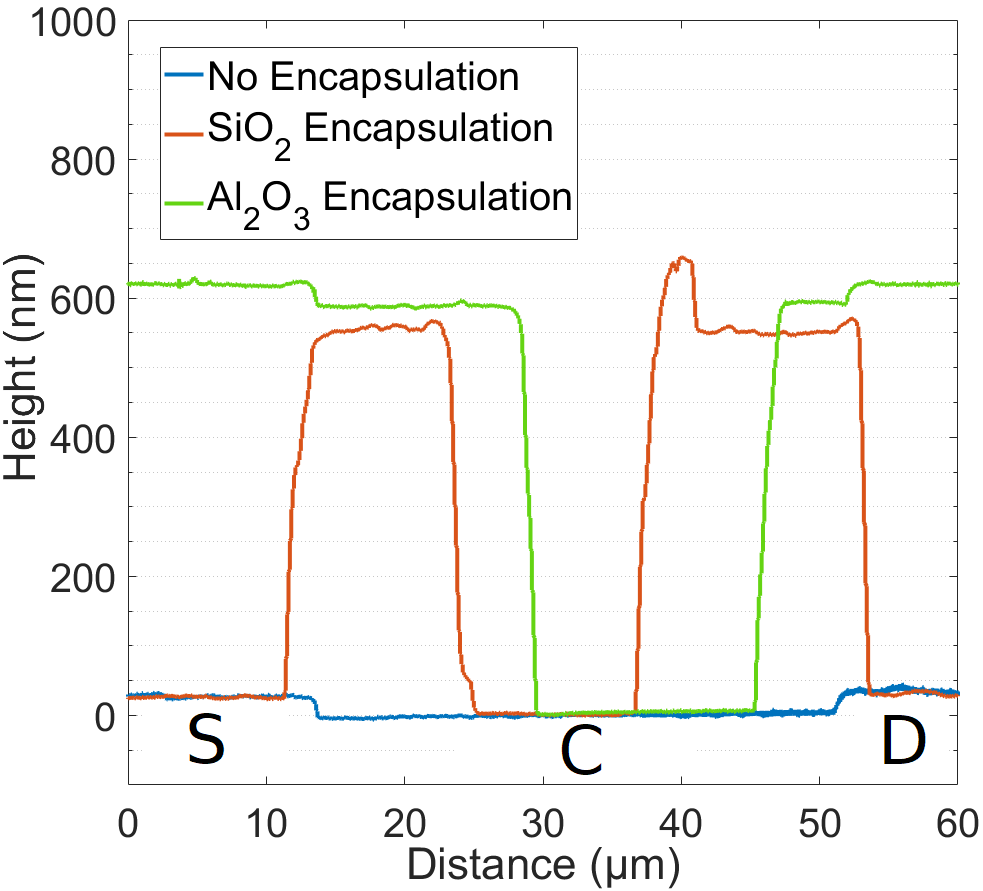
\includegraphics{figures/ch4/Dielectric_Profile_comparison_edit.png}

}

}

\end{minipage}%
%
\begin{minipage}[t]{0.01\linewidth}

{\centering 

~

}

\end{minipage}%
%
\begin{minipage}[t]{0.03\linewidth}

{\centering 

\raisebox{-\height}{

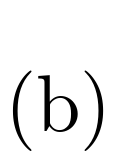
\includegraphics{figures/(b).png}

}

}

\end{minipage}%
%
\begin{minipage}[t]{0.01\linewidth}

{\centering 

~

}

\end{minipage}%
%
\begin{minipage}[t]{0.42\linewidth}

{\centering 

\raisebox{-\height}{

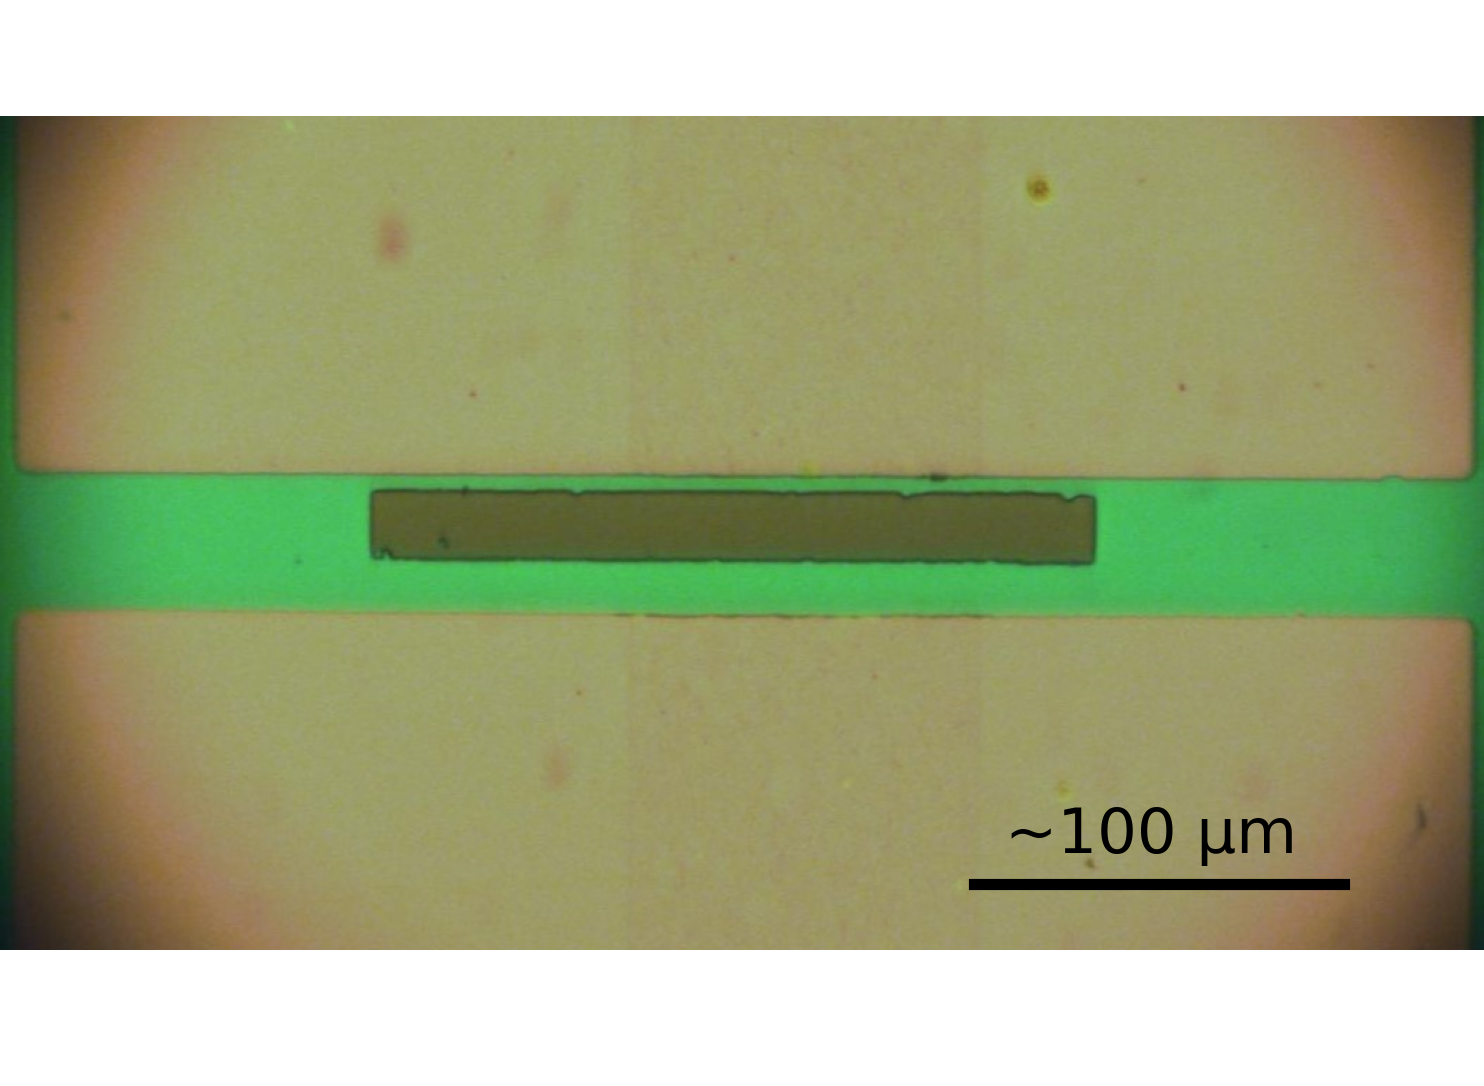
\includegraphics{figures/ch4/al2o3_encapsulation.png}

}

}

\end{minipage}%
%
\begin{minipage}[t]{0.01\linewidth}

{\centering 

~

}

\end{minipage}%

\caption{\label{fig-dektat-dielectric-layer}A profile comparison of
dielectric materials used for encapsulation is shown in (a), alongside a
microscope image of a device encapsulated with aluminium oxide in (b).
Note that the layer thicknesses in (a) were from initial tests of the
process and are used for illustrative purposes. S is source electrode, D
is drain electrode and C is the channel region.}

\end{figure}

The initial attempt at fabricating a dielectric encapsulation layer used
silicon dioxide as the dielectric. However, silicon dioxide adheres
poorly to gold without an metallic adhesive layer present, as shown in
Figure~\ref{fig-dektat-dielectric-layer} (a). Aluminium oxide was chosen
as an alternative as it sticks well to bulk electrode materials, is heat
and chemical resistant, has a relatively high dielectric constant and is
bio-compatible \autocite{Guarnieri2014,Albarghouthi2022,Kolodzey2000}.
Figure~\ref{fig-dektat-dielectric-layer} (b) shows the aluminium oxide
successfully adhered to the electrodes and
Figure~\ref{fig-dektat-dielectric-layer} (a) shows the layer had a clean
profile after lift-off. Unfortunately, when aluminium oxide layers which
were thicker than \(\sim\) 100 nm were deposited, a significant drop in
channel mobility occurred after encapsulation. This drop was signficant
enough to make devices unsuitable for sensing. Meanwhile, devices with
encapsulation \(\sim\) 100 nm thick had significant gate current leakage
through the encapsulation layer when liquid-gated. This leakage was
present even when AZ\(^\circledR\) nLOF 2020 was used when patterning
electrodes to avoid edge spikes (as discussed in
Section~\ref{sec-electrodes}). Furthermore, aluminium oxide should not
be subsequently exposed to its etchant TMAH, meaning it was difficult to
completely remove residual photoresist from device channels after
encapsulation. Alternative approaches to high-dielectric ceramic
encapsulation are discussed in \textbf{?@sec-future-work-fabrication}.

\hypertarget{characterisation-of-carbon-nanotube-and-graphene-field-effect-transistors}{%
\section{Characterisation of Carbon Nanotube and Graphene Field-Effect
Transistors}\label{characterisation-of-carbon-nanotube-and-graphene-field-effect-transistors}}

\hypertarget{sec-afm-characterisation}{%
\subsection{Atomic Force Microscopy}\label{sec-afm-characterisation}}

Atomic force microscopy in this thesis was taken using a Nanosurf
NaioAFM in dynamic force mode (also known as tapping mode, oscillating
mode, acoustic AC mode or intermittent-contact mode). An ACLA probe
(AppNano) was used with a tip diameter of 12 nm, height of \(14-16\) µm
and a nominal cantilever spring constant of 58 N/m. All atomic force
microscopy was performed with the Nanosurf NaioAFM on a stablising table
under a Faraday cage to minimise mechanical and electromagnetic
interference. A 256 \(\times\) 256 pixel resolution was typically used.
Imaging was performed in air at room temperature. Atomic force
microscope (AFM) images could not be taken from the small exposed
channel region on the encapsulated devices, so were instead taken on a
representative carbon nanotube or graphene film sample fabricated on the
same wafer as the device being tested. Moisture adversely affected the
AFM imaging process. Therefore, films functionalised with biological
materials were washed with DI water and gently dried with N\(_2\) before
atomic force microscope images were taken. The open source data analysis
software Gwyddion (version 2.59) was used to analyse AFM images. This
included levelling the background with the polynomial background removal
function, removing scarring and zeroing the z-scale.

\hypertarget{sec-fluorescence-characterisation}{%
\subsection{Fluorescence
Microscopy}\label{sec-fluorescence-characterisation}}

Fluorescence microscopy was performed using an Olympus BX63 fluorescence
microscope controlled using cellSens imaging software. Microscope
objectives used were all Olympus UPLSAPO/UPlanSApo, apochromat
objectives which compensate for spherical and chromatic aberrations.
Objectives had infinite aperture and a field number of 26.5. Filter
cubes used included the Olympus FITC filter (excitation wavelength
range: \(467-498\) nm, emission wavelength range: \(513-556\) nm), Texas
Red (excitation wavelength range: \(542-582\) nm, emission wavelength
range: \(604-644\) nm) and GFP (excitation wavelength range: \(604-644\)
nm, emission wavelength range: \(502-538\) nm). The ISO sensitivity was
kept at the lowest available setting, ISO200. All microscopy was
performed in darkness with the screen turned away from the microscope.
To ensure photobleaching did not adversely affect imaging, images were
taken soon after initial exposure to fluorescence and taking repeated
photos of the same region was avoided. Various useful and thorough
introductions to fluorescence microscopy can be found online
\autocite{Nikon,Zeiss}.

\hypertarget{sec-raman-characterisation}{%
\subsection{Raman Spectroscopy}\label{sec-raman-characterisation}}

Raman spectroscopy was performed with a HORIBA Jobin Yvon LabRAM HR800
Raman spectrometer. The wavelength and power used for laser excitation
of samples were 514 nm and 1 mW respectively. Spectra were taken with a
1800 line holographic grating with a hole size of 300 µm. A accumulation
time of 20 seconds was used when taking spectra. Each spectrum was
recorded twice at ten positions within a 40 µm \(\times\) 100 µm
rectangular region on a carbon nanotube film, with a vertical spacing of
10µm and horizonal spacing of 20 µm between each position. Spectra were
collected over two wavenumber ranges at each position, with the first
range between 100 cm\(^{-1}\) and 650 cm\(^{-1}\), and the second
between 1300 cm\(^{-1}\) and 1650 cm\(^{-1}\). Data collected at the
final, tenth position was often much noiser than all other measurements
taken due to an unclear experimental issue, and this data was therefore
discarded.

\hypertarget{sec-electrical-characterisation}{%
\subsection{Electrical
Characterisation}\label{sec-electrical-characterisation}}

Both liquid-gated and back-gated measurements were taken of carbon
nanotube and graphene devices. All measurement setups used had the same
basic configuration, with two source measure units (SMUs) attached to
the source and gate. \(V_{ds}\) was applied between the source SMU (SMU
1) and the drain SMU (SMU 2), while \(V_{g}\) was applied between the
gate SMU (SMU 3) and the drain SMU. The drain SMU was held at 0 V or
connected to a ground plane. Drain current \(I_{d}\) was measured at the
drain SMU, and gate leakage current \(I_{g}\) was measured at the gate
SMU. Voltage from the source and gate SMUs was either kept constant or
varied, with only one SMU voltage varied at a time. Three different
measurement setups were used for taking these measurements, the Agilent
(Keysight/HP) 4156C semiconductor parameter analyser, the Keysight
B1500A semiconductor device analyser, and a National Instruments NI-PXIe
modular measurement system with a 8 GB PXIe-8821 controller and two
NI-4138 source measure units in the system chassis.

\begin{figure}

{\centering 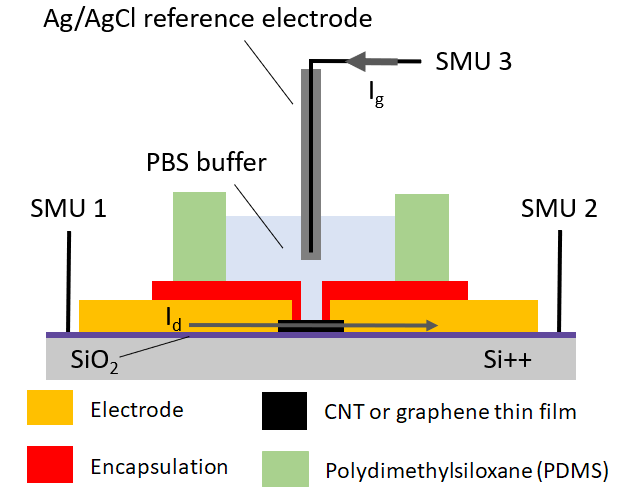
\includegraphics{figures/ch4/liquid-gate-schematic.png}

}

\caption{\label{fig-liquid-gate}A liquid-gated device schematic showing
electrical connections to the three source measure units, SMU 1, SMU 2
and SMU 3.}

\end{figure}

Liquid-gated measurements were taken using the configuration shown in
Figure~\ref{fig-liquid-gate}. Ag/AgCl standard electrodes were used as
the liquid-gate electrode. The electrode was submerged in 80 µL of PBS
buffer in a polydimethylsiloxane (PDMS) `well' \(-\) a flexible
structure used to contain the electrolyte solution \(-\) with outer
dimensions of 12 mm \(\times\) 6 mm \(\times\) 6 mm. This PDMS well was
sonicated in isopropanol for 10 min and thoroughly N\(_2\) dried before
use. Microscope images of the PDMS surface before and after this
cleaning step are shown in Figure~\ref{fig-PDMS-clean} (a) and
Figure~\ref{fig-PDMS-clean} (b) respectively. The end of Ag/AgCl
standard electrode to be submerged was rinsed in DI water and left to
sit in DI water for 15 minutes before each characterisation. When using
the Agilent 4156C semiconductor parameter analyser or Keysight B1500A
semiconductor device analyser for liquid-gated measurements, a
Faraday-caged Rucker and Kolls 666 probe station with micromanipulators
was used to contact the devices. When using the National Instruments
NI-PXIe system for liquid-gated measurements, a custom-made chip carrier
with spring-loaded, pointed-tip, gold-coated pogo pins was used.

\begin{figure}

\begin{minipage}[t]{0.03\linewidth}

{\centering 

\raisebox{-\height}{


\includegraphics{figures/(a).png}

}

}

\end{minipage}%
%
\begin{minipage}[t]{0.01\linewidth}

{\centering 

~

}

\end{minipage}%
%
\begin{minipage}[t]{0.45\linewidth}

{\centering 

\raisebox{-\height}{

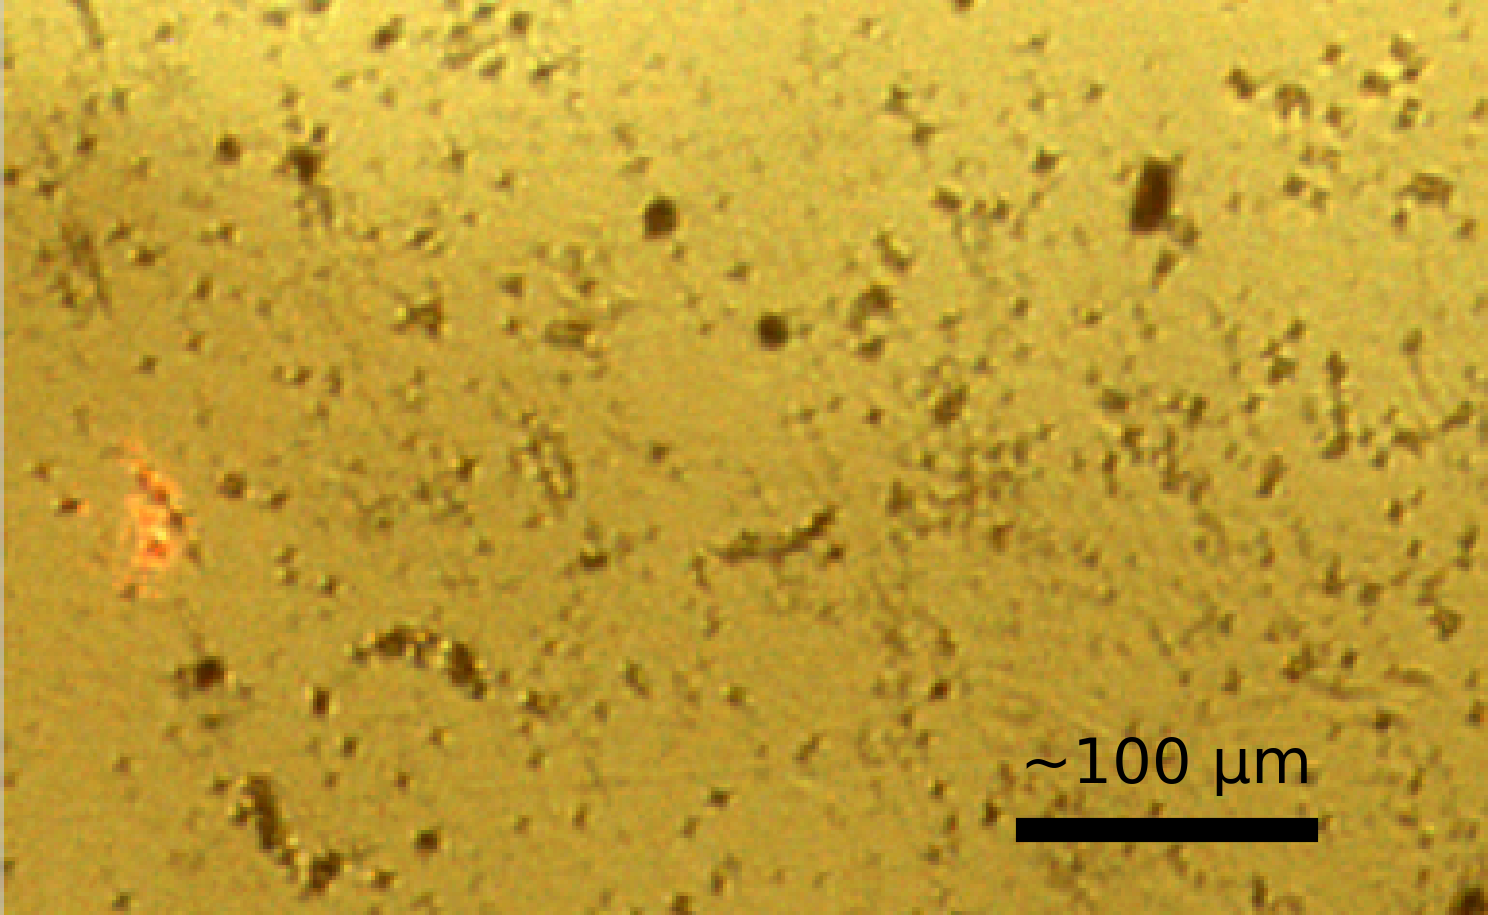
\includegraphics{figures/ch4/PDMS_dirty.png}

}

}

\end{minipage}%
%
\begin{minipage}[t]{0.01\linewidth}

{\centering 

~

}

\end{minipage}%
%
\begin{minipage}[t]{0.03\linewidth}

{\centering 

\raisebox{-\height}{

\includegraphics{figures/(b).png}

}

}

\end{minipage}%
%
\begin{minipage}[t]{0.01\linewidth}

{\centering 

~

}

\end{minipage}%
%
\begin{minipage}[t]{0.45\linewidth}

{\centering 

\raisebox{-\height}{

\includegraphics{figures/ch4/PDMS_clean.png}

}

}

\end{minipage}%
%
\begin{minipage}[t]{0.01\linewidth}

{\centering 

~

}

\end{minipage}%

\caption{\label{fig-PDMS-clean}Microscope images of the surface of a
PDMS well before (a) and after (b) isopropanol (IPA) sonication for 10
minutes.}

\end{figure}

Back-gated measurements were taken with a copper plane placed underneath
the Si/SiO\(_2\) wafer and connected to SMU 3. The Agilent 4156C
Semiconductor Parameter Analyser and Keysight B1500A Semiconductor
Device Analyser were used for back-gated measurements of devices within
the vapour delivery system device chamber. When the lid of this chamber
was tightly sealed, it acted a Faraday cage for another custom-made chip
carrier with spring-loaded gold-coated pogo pins, able to contact four
channel electrode pairs at once. The silicon back of the device was
pressed by the pins against a copper block, connected to the gate SMU.
The design of the chamber chip carrier printed circuit board (PCB) is
shown in Figure~\ref{fig-device-interface} (a). The 0.5 mm through holes
connect the PTFE-coated wires, which then connect to the output cable,
while the 1.75 mm through holes are for attaching the sleeves of gold
pogo pins. These pogo pins contact the device within the chamber. 2 ×
2.5 mm solder pads have been placed around the 1.75 mm throughholes for
better contact with the pogo pin sleeves. The circuit board was placed
within two layers of PTFE casing for mounting and protection from vapour
within the chamber. The wired interface is shown in
Figure~\ref{fig-device-interface} (b), where the PTFE block is
protecting the encased circuit board. The Faraday-cage Rucker and Kolls
probe station was used for all back-gated measurements taken outside the
vapour sensing chamber.

\begin{figure}

\begin{minipage}[t]{0.03\linewidth}

{\centering 

\raisebox{-\height}{

\includegraphics{figures/(a).png}

}

}

\end{minipage}%
%
\begin{minipage}[t]{0.03\linewidth}

{\centering 

~

}

\end{minipage}%
%
\begin{minipage}[t]{0.91\linewidth}

{\centering 

\raisebox{-\height}{

\includegraphics{figures/ch4/chip_PCB.png}

}

}

\end{minipage}%
%
\begin{minipage}[t]{0.03\linewidth}

{\centering 

~

}

\end{minipage}%
\newline
\begin{minipage}[t]{0.03\linewidth}

{\centering 

\raisebox{-\height}{

\includegraphics{figures/(b).png}

}

}

\end{minipage}%
%
\begin{minipage}[t]{0.03\linewidth}

{\centering 

~

}

\end{minipage}%
%
\begin{minipage}[t]{0.91\linewidth}

{\centering 

\raisebox{-\height}{

\includegraphics{figures/ch4/device_interface.png}

}

}

\end{minipage}%
%
\begin{minipage}[t]{0.03\linewidth}

{\centering 

~

}

\end{minipage}%

\caption{\label{fig-device-interface}The circuit board schematic for the
interface between the sensor device and output signal cable leaving the
delivery system chamber is shown in (a). The interface as constructed is
shown in (b). This electronic interface was designed and put together by
Rifat Ullah, School of Chemical and Physical Sciences, Te Herenga Waka -
Victoria University of Wellington.}

\end{figure}

Custom programs for National Instruments LabView 2017 were used for
measurements from the Agilent 4156C Semiconductor Parameter Analyser and
the National Instruments NI-PXIe. Keysight EasyEXPERT software was used
for characterisation with the Keysight B1500A Semiconductor Device
Analyser. Liquid-gated transfer characteristics of carbon nanotube FETs
were measured at V\(_{\mathrm{ds}}\) = 100 mV and liquid-gated transfer
characteristics of graphene FETs were measured at V\(_{\mathrm{ds}}\) =
1 V, where V\(_{\mathrm{lg}}\) was swept between -0.5 V and 1 V in both
the forward and reverse direction with a step size of either 10 or 20
mV. Backgated transfer characteristics of carbon nanotube FETs were
either measured at V\(_{\mathrm{ds}}\) = 100 mV or V\(_{\mathrm{ds}}\) =
1 V, where V\(_{\mathrm{bg}}\) was swept between -5 V and 5 V or -10 V
and 10 V in the forward and reverse directions with a step size of 50 mV
or 100 mV.

A liquid-gated setup was used for aqueous-phase sensing and a back-gated
setup in the vapour delivery system was used for vapour-phase sensing.
Sensing measurements were performed with constant source-drain and gate
voltages. The gate voltage used was chosen by locating the subthreshold
region of the device transfer characteristics and choosing a voltage
that fell within this region, usually V\(_{\mathrm{g}}\) = 0 V. Using
the NI-PXIe with the PXIe-2737 module, eight-channel multiplexed current
measurements could be taken in rapid succession. An integration time of
200 or 400 ms was used for sampling with each channel, with the actual
sampling rate set by the NI-PXIe. In practice this meant a sampling rate
of 1.81 s (for 200 ms integration time) or 3.41 s (for 400 ms
integration time) for any given channel. A 200 ms integration time meant
the time between samples from successive channels varied between
\(220 ms-230\) ms, while a 400 ms integration time meant the time
between samples was consistently 426 ms. The Keysight equipment used a
constant 1 s sampling interval.

\hypertarget{aqueous-sensing}{%
\subsubsection*{Aqueous Sensing}\label{aqueous-sensing}}
\addcontentsline{toc}{subsubsection}{Aqueous Sensing}

Before the sensing process, 200 µL of PBS was added to the PDMS well and
100-120 µL of PBS was removed. This initial step was performed to wet
the sides of the PDMS well, and check that the attachment of the PDMS
well to the device would not unseal when larger volumes of PBS were
added during sensing. Before any sensing measurement, a transfer
characteristic curve was taken of the liquid-gated device. The initial
amount of buffered electrolyte in the well was 100 µL, unless specified
otherwise.

From Feburary 2022 onwards, the standard sensing addition series used
comprised of a `control series' and an `analyte sensing series'. The
control series was performed as part of each sensing experiment to test
for unwanted responses to electrolyte and to allow baseline drift to
settle. The total control series interval was 1800 s. Electrolyte
additions of 20 µL were made at 100 s, 200 s and 300 s, while
electrolyte subtractions of 20 µL were made at 400 s, 500 s and 600 s.
Immediately after the control series, a sensing sequence was performed
as part of the same continuous measurement set. An initial electrolyte
addition was performed at 2100s, to confirm no changes occurred during
the control series that would interfere with sensing. Unless specified
otherwise, five analyte additions were then made with a time spacing of
300 s, at 2400 s, 2700 s, 3000 s, 3300 s and 3600 s. The experimental
series was set to finish at 4000 s. The exact timings, analyte
concentrations and gate voltage used in a given sensing sequence are
discussed alongside the relevant experimental results.

\hypertarget{vapour-sensing}{%
\subsubsection*{Vapour Sensing}\label{vapour-sensing}}
\addcontentsline{toc}{subsubsection}{Vapour Sensing}

Various vapour exposure procedures were used during sensing
measurements. These procedures were performed with the vapour delivery
system, and are described in further detail in
\textbf{?@sec-vapour-sensing-biosensors} and
\textbf{?@sec-pristine-characteristics}.

\hypertarget{summary}{%
\section{Summary}\label{summary}}

Several approaches were trialled when depositing a carbon nanotube
network for the fabrication of transistor devices, which fall under the
general categories of solvent-deposited, surfactant-deposited and
surfactant-deposited with steam present. Standard photolithographic
methods were used to successfully fabricate carbon nanotube and graphene
field effect transistor devices. A range of photolithography types and
electrode/encapsulation materials were trialled to find the optimal
device composition for sensing. Atomic force microscopy, fluorescence
microscopy and a variety of electrical measurement setups were used to
characterise the devices. Pristine device characteristics can be found
in \textbf{?@sec-pristine-characteristics}, while functionalised device
characteristics can be found in
\textbf{?@sec-noncovalent-functionalisation} and
\textbf{?@sec-biosensing-iORs}.

\bookmarksetup{startatroot}

\hypertarget{references}{%
\chapter*{References}\label{references}}
\addcontentsline{toc}{chapter}{References}

\markboth{References}{References}

\printbibliography[heading=none]

\cleardoublepage
\phantomsection
\addcontentsline{toc}{part}{Appendices}
\appendix

\hypertarget{vapour-system-hardware}{%
\chapter{Vapour System Hardware}\label{vapour-system-hardware}}


\hypertarget{tbl-vapour-sensor-components}{}
\begin{longtable}[t]{>{\raggedright\arraybackslash}p{5.5cm}>{\raggedright\arraybackslash}p{4.5cm}>{\raggedright\arraybackslash}p{3.75cm}}
\caption{\label{tbl-vapour-sensor-components}Major components used in construction of the vapour delivery system
described in this thesis. }\tabularnewline

\toprule
Description & Part No. & Manufacturer\\
\midrule
Mass flow controller, 20 sccm full scale & GE50A-013201SBV020 & MKS Instruments\\
Mass flow controller, 200 sccm full scale & GE50A-013202SBV020 & MKS Instruments\\
Mass flow controller, 500 sccm full scale & FC-2901V & Tylan\\
Analogue flowmeter, 240 sccm max. flow & 116261-30 & Dwyer\\
Micro diaphragm pump & P200-B3C5V-35000 & Xavitech\\
\addlinespace
Analogue flow controller, for micro diaphragm pump & X3000450 & Xavitech\\
10 mL Schott bottle & 218010802 & Duran\\
PTFE connection cap system & Z742273 & Duran\\
Baseline VOC-TRAQ flow cell, purple & 043-950 & Ametek Mocon\\
Baseline VOC-TRAQ flow cell, red & 043-951 & Ametek Mocon\\
\addlinespace
Humidity and temperature sensor & T9602-5-A & Telaire\\
Enclosure, for humidity and temperature sensor & MC001189 & Multicomp Pro\\
\bottomrule
\end{longtable}

\hypertarget{python-code-for-data-analysis}{%
\chapter{Python Code for Data
Analysis}\label{python-code-for-data-analysis}}

\hypertarget{code-repository}{%
\section{Code Repository}\label{code-repository}}

The code used for general analysis of field-effect transistor devices in
this thesis was written with Python 3.8.8. Contributors to the code used
include Erica Cassie, Erica Happe, Marissa Dierkes and Leo Browning. The
code is located on GitHub and the research group OneDrive, and is
available on request.

\hypertarget{sec-histogram-analysis}{%
\section{Atomic Force Microscope Histogram
Analysis}\label{sec-histogram-analysis}}

The purpose of this code is to analyse atomic force microscope (AFM)
images of carbon nanotube networks in .xyz format taken using an atomic
force microscope and processed in Gwyddion (see
Section~\ref{sec-afm-characterisation}). It was originally designed by
Erica Happe in Matlab, and adapted by Marissa Dierkes and myself for use
in Python. The code imports the .xyz data and sorts it into bins 0.15 nm
in size for processing. To perform skew-normal distribution fits, both
\emph{scipy.optimize.curve\_fit} and \emph{scipy.stats.skewnorm} modules
are used in this code.

\hypertarget{sec-raman-analysis}{%
\section{Raman Spectroscopy Analysis}\label{sec-raman-analysis}}

The purpose of this code is to analyse a series of Raman spectra taken
at different points on a single film (see
Section~\ref{sec-raman-characterisation}). Data is imported in a series
of tab-delimited text files, with the low wavenumber spectrum (100
cm\(^{-1} - 650\) cm\(^{-1}\)) and high wavenumber spectrum (1300
cm\(^{-1} - 1650\) cm\(^{-1}\)) imported in separate datafiles for each
scan location.

\hypertarget{sec-field-effect-transistor-analysis}{%
\section{Field-Effect Transistor
Analysis}\label{sec-field-effect-transistor-analysis}}

The purpose of this code is to analyse electrical measurements taken of
field-effect transistor (FET) devices. Electrical measurements were
either taken from the Keysight 4156C Semiconductor Parameter Analyser,
National Instruments NI-PXIe or Keysight B1500A Semiconductor Device
Analyser as discussed in Section~\ref{sec-electrical-characterisation};
the code is able to analyse data in .csv format taken from all three
measurement setups. The main Python file in the code base consists of
three related but independent modules: the first analyses and plots
sensing data from the FET devices, the second analyses and plots
transfer characteristics from channels across a device, and the third
compares individual channel characteristics before and after a
modification or after each of several modifications. The code base also
features a separate config file and style sheet which govern the
behaviour of the main code. The code base was designed collaboratively
by myself and Erica Cassie over GitHub using the Sourcetree Git GUI.


\backmatter
\printbibliography[title=References]


\end{document}
